%% \chapter[htoc-titlei][hhead-titlei]{htitlei}
%% -----------------------------------------------------------------------------
\chapter[The LHC and the \atlas\ experiment][The LHC and \atlas]
        {The Large Hadron Collider and the \atlas\ experiment}
\label{ch:lhc}

\begin{quote}
  As the name suggests, the Large Hadron Collider (LHC) is a particle collider,
  which collides particles at very high energies.
  There are four major experiments, including \atlas, which collect and study
  data generated from these particle collisions in an effort to study
  the properties of nature, and search for signs of physics beyond the Standard
  Model.
  This chapter gives a brief introduction to the LHC machine, and the
  \atlas\ experiment.
\end{quote}

%% ------------------------------------------------------------------------------
\FloatBarrier
\section{The LHC machine}
\label{sec:lhc}

The LHC~\cite{cern-jinst-lhc} is circular particle accelerator, with a
circumference of 27~km, built 100~m underground, underneath the French-Swiss
border near the city of Geneva, Switzerland, shown in
Figure~\ref{fig:lhc_aerial}.
The LHC is operated by the European Organization for Nuclear Research
(CERN~\footnote{Conseil Europ\'een pour la Recherche Nucl\'eaire}).
The LHC became fully operational in 2010, providing proton-proton collisions
to the experiments along the ring at an unprecedented center-of-mass energy
of 7~\TeV.
In 2012, the energy was increased to 8~\TeV.

\begin{figure}[ht]
  \centering
  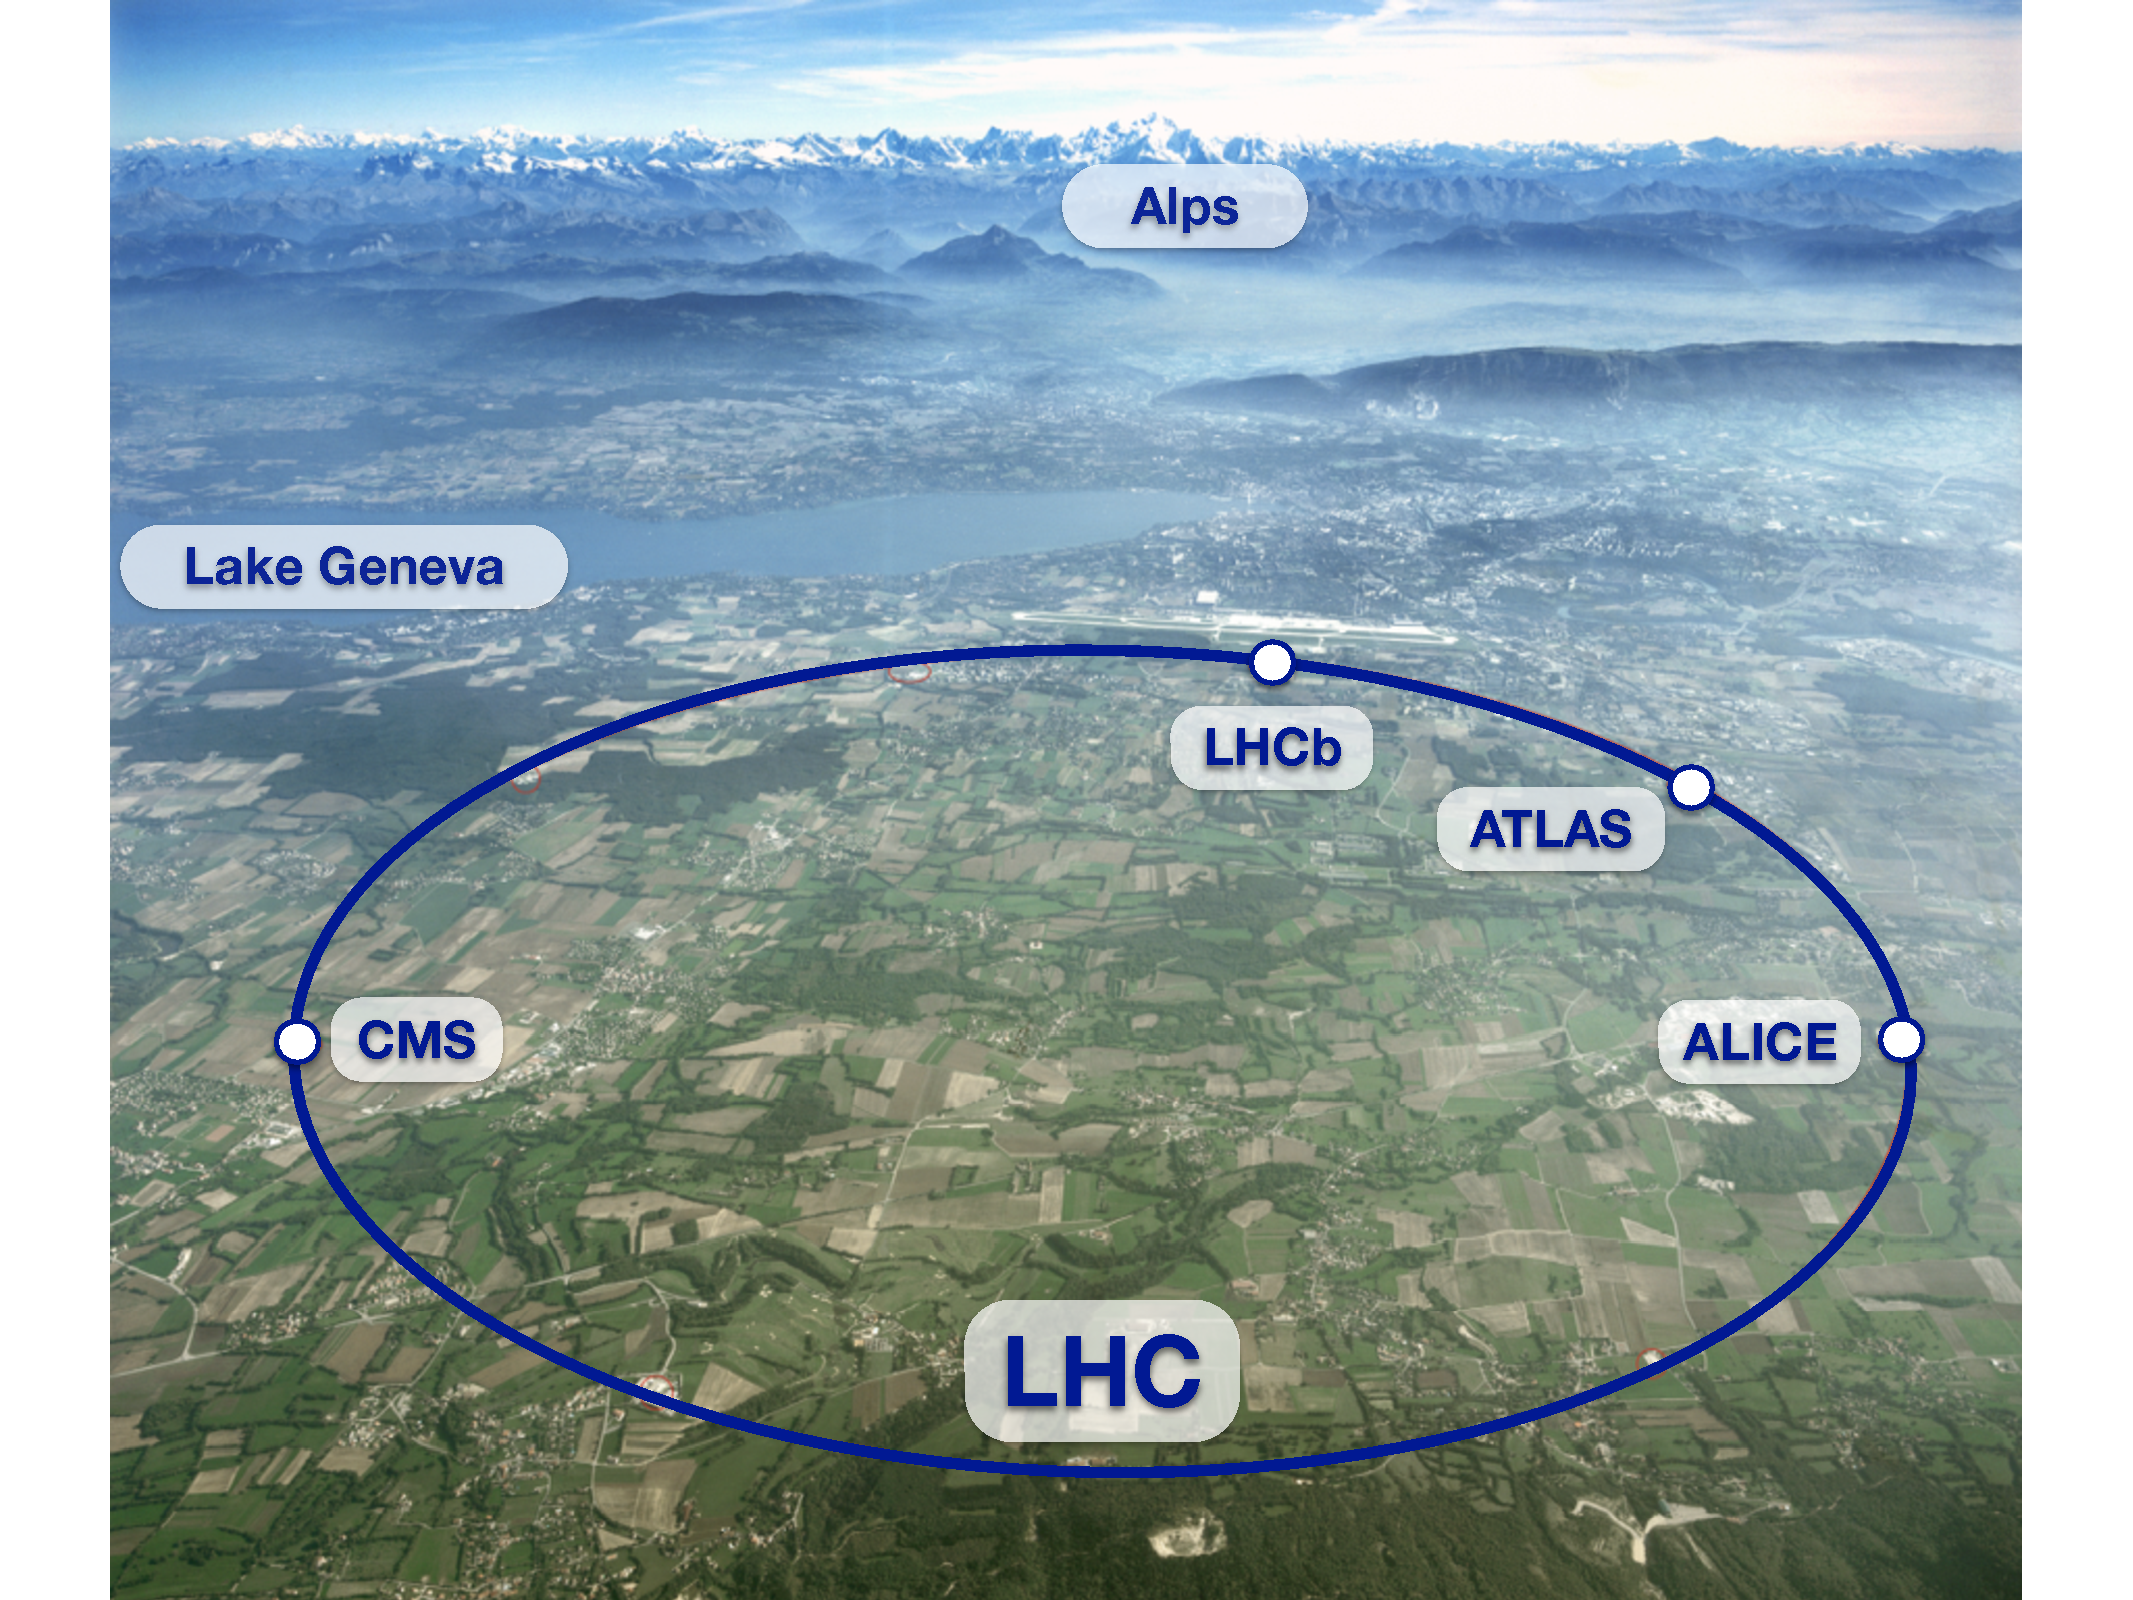
\includegraphics[width=\textwidth, clip=true, trim=0 0 1cm 0]
    {figs/lhc/lhc_aerial.pdf}
  \caption{
    Areal view of the Geneva area with an overlaid drawing of the LHC
    and experiments~\cite{lhc_aerial}.
  }
  \label{fig:lhc_aerial}
\end{figure}

Four major experiments are positioned around the LHC to collect and analyze
data from the hadron collisions.
The experiments include \atlas~\cite{cern-jinst-atlas},
\cms~\cite{cern-jinst-cms}, \alice~\cite{cern-jinst-alice}, and
\lhcb~\cite{cern-jinst-lhcb}.
\atlas\ and \cms\ are designed to be ``general purpose experiments,'' searching
for physics beyond the Standard Model which may present itself in may ways.
The two experiments complement each other by providing independent results,
which can be verified against the each other.
\alice\ is designed to study the heavy ion (lead nuclei) collisions, studying
the properties of quark-gluon plasma.
The \lhcb\ experiment is primarily interested in studying the physics of
$b$-hadrons.

%% ------------------------------------------------------------------------------
\FloatBarrier
\subsection{CERN accelerator complex}
\label{sec:accelerator_complex}

The LHC is only the final stage in a series of accelerators, operated by CERN,
used to provide high energy particle collisions.
For proton-proton collisions, protons begin in the Linac 2 linear
accelerator, where they are accelerated to an energy of 50~\MeV\ per proton.
From there, they are fed through several circular accelerators, including
the Proton Synchrotron Booster (PSB), Proton Synchrotron (PS), and the Super
Proton Synchrotron (SPS), where the protons are accelerated to energies of
1.4~\GeV, 25~\GeV, and 450~\GeV\ respectively.
At this stage, the protons are injected into the LHC accelerator, where 
in 2012, they were accelerated to an energy of 4~\TeV\ per proton, and finally
collided.
A schematic of the CERN accelerator complex, and how they link to one another
is shown in Figure~\ref{fig:cern_complex}.

\begin{figure}[ht]
  \centering
  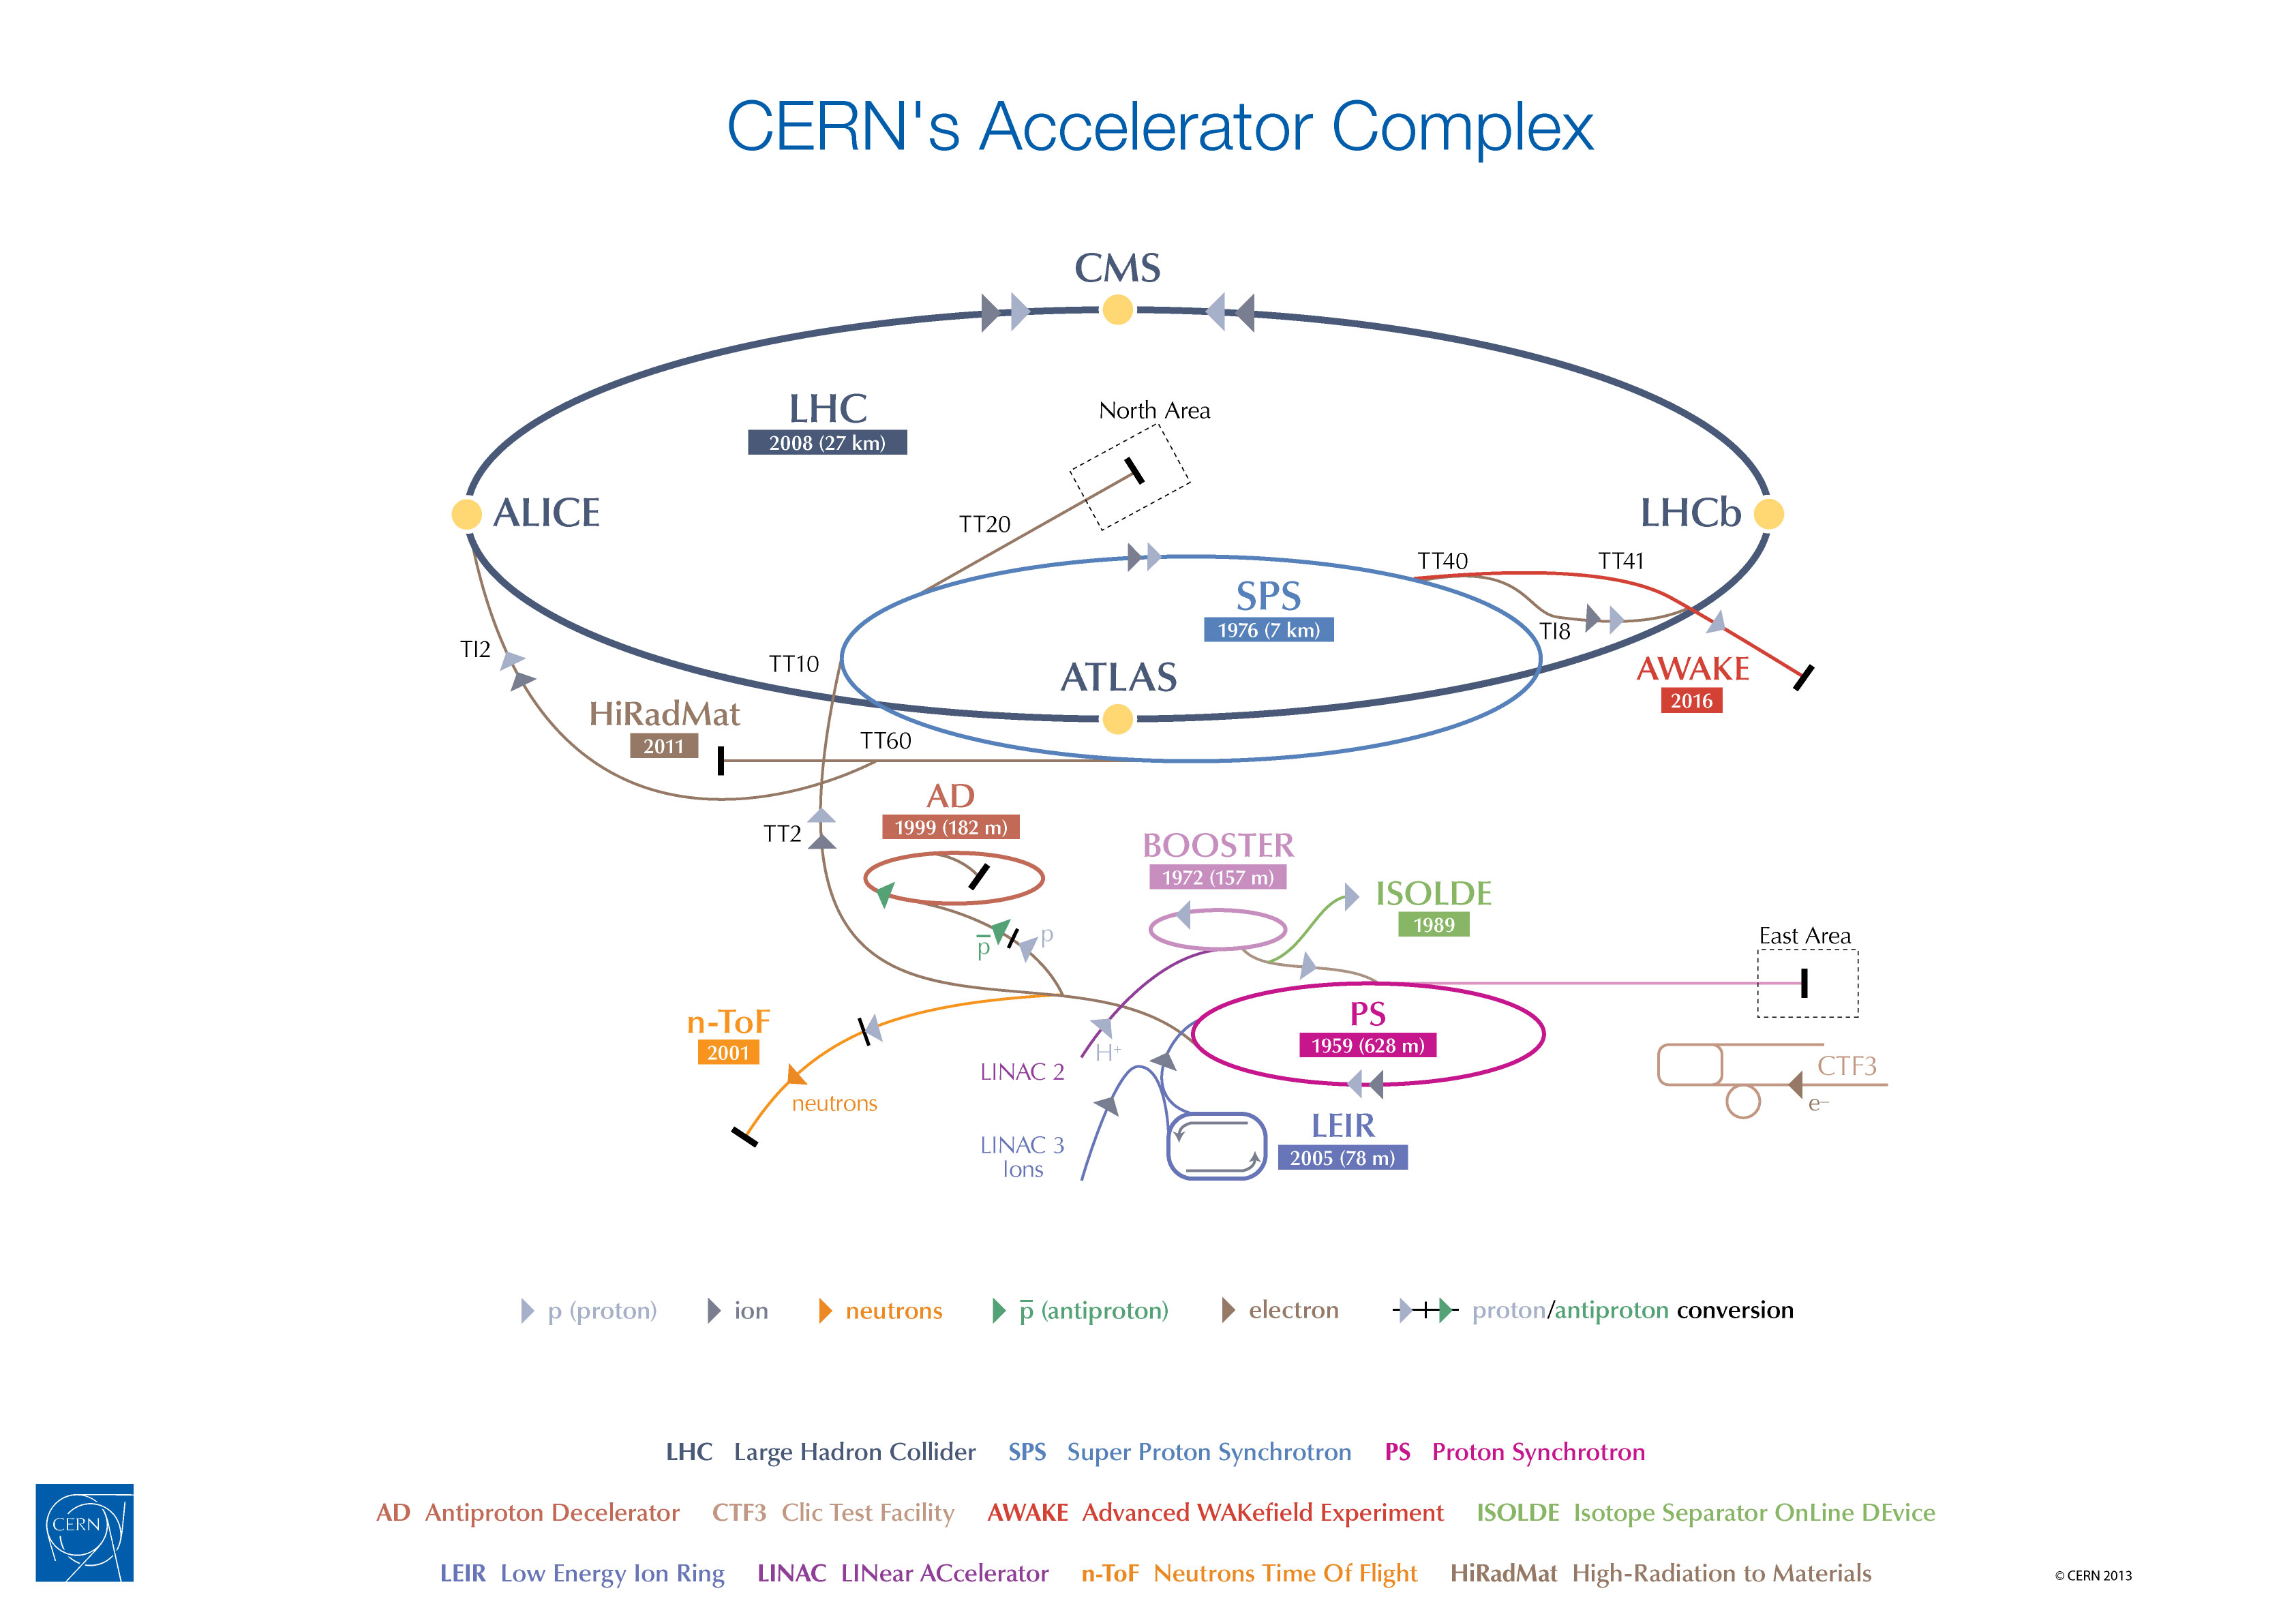
\includegraphics[width=\textwidth, clip=true, trim=15cm 0 15cm 10cm]
    {figs/lhc/accelerator_complex.jpg}
  \caption{
    Schematic view of the CERN accelerator complex~\cite{Marcastel:1621583}.
  }
  \label{fig:cern_complex}
\end{figure}

%% ------------------------------------------------------------------------------
\FloatBarrier
\subsection{LHC beam conditions}
\label{sec:beam_conditions}

Rather than a constant stream of protons, the protons in the LHC are separated
into over 1000 bunches, each containing over $10^{11}$ protons.
In each of the interaction points around the LHC ring, proton bunches cross
onces every 50~ns, where each crossing leads to potential collisions between
the constituent protons.
The instantaneous luminosity of collisions in these bunch crossings is given by
\begin{equation}
  \mathcal{L}_\mathrm{instantaneous} =
  \frac{N_{1}N_{2} n_b f_\mathrm{rev}}
  {4\pi \sigma_{x} \sigma_{y}}
  F,
\end{equation}
where $N_{1,2}$ are the number of protons per bunch, $n_b$ is the number of
bunches, $f_\mathrm{rev}$ is the frequency at which the protons are revolution
frequency, $\sigma_{x,y}$ is the width of the beam in the transverse directions,
and $F$ is a reduction factor, accounting for the fact that the beams cross
at an angle, rather than head-on.
As the proton beams circulate, and undergo collisions, they tend to spread out,
increasing $\sigma_{x,y}$, and reducing the instantaneous luminosity over time.
Typically, once the LHC is filled with proton beams, and accelerated to their
full energy, they are circulated for several hours before they are dumped, and
the accelerator is filled again.

\begin{figure}
  \centering
  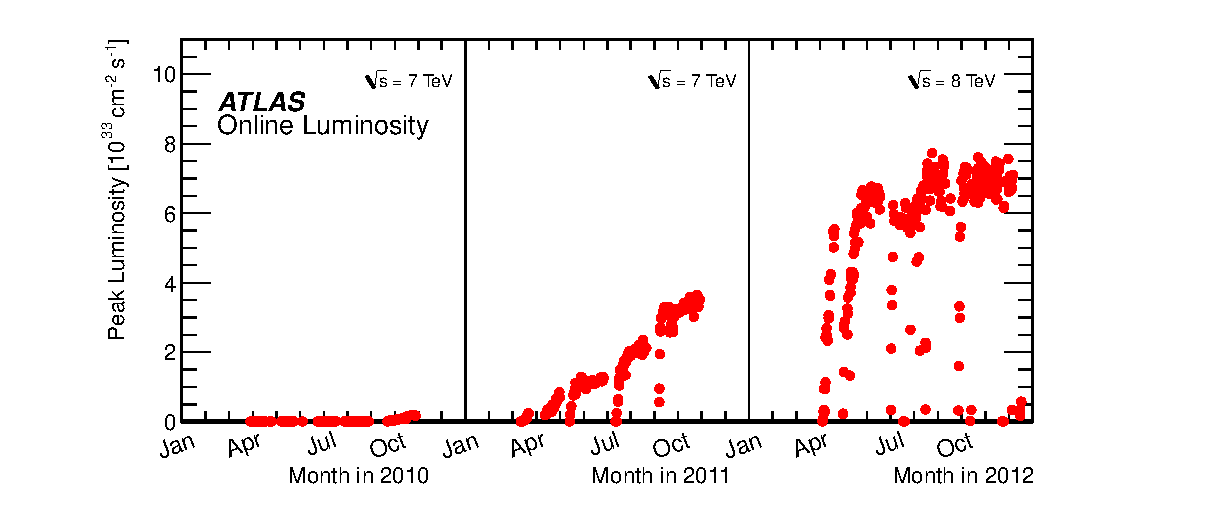
\includegraphics[width=0.9\textwidth]{figs/lhc/lumivstime.eps}
  \caption{
    Instantaneous luminosity collected by the ATLAS detector throughout
    Run 1~\cite{atlas-lumi}.
  }
  \label{fig:inst_lumi_vs_time}
\end{figure}

Figure~\ref{fig:inst_lumi_vs_time} shows the instantaneous luminosity of
proton-proton collisions provided to ATLAS by the LHC increased throughout the
running period as the machine was thoroughly tested and better understood.
This is accomplished by adding more protons, and squeezing the beams into
a smaller area for the collisions.
The higher instantaneous luminosity allowed for faster data collection in later
running periods, but came at the cost of a larger number of interactions per
crossing, seen in Figure~\ref{fig:int_lumi_vs_time_and_pileup}.

\begin{figure}
  \centering
  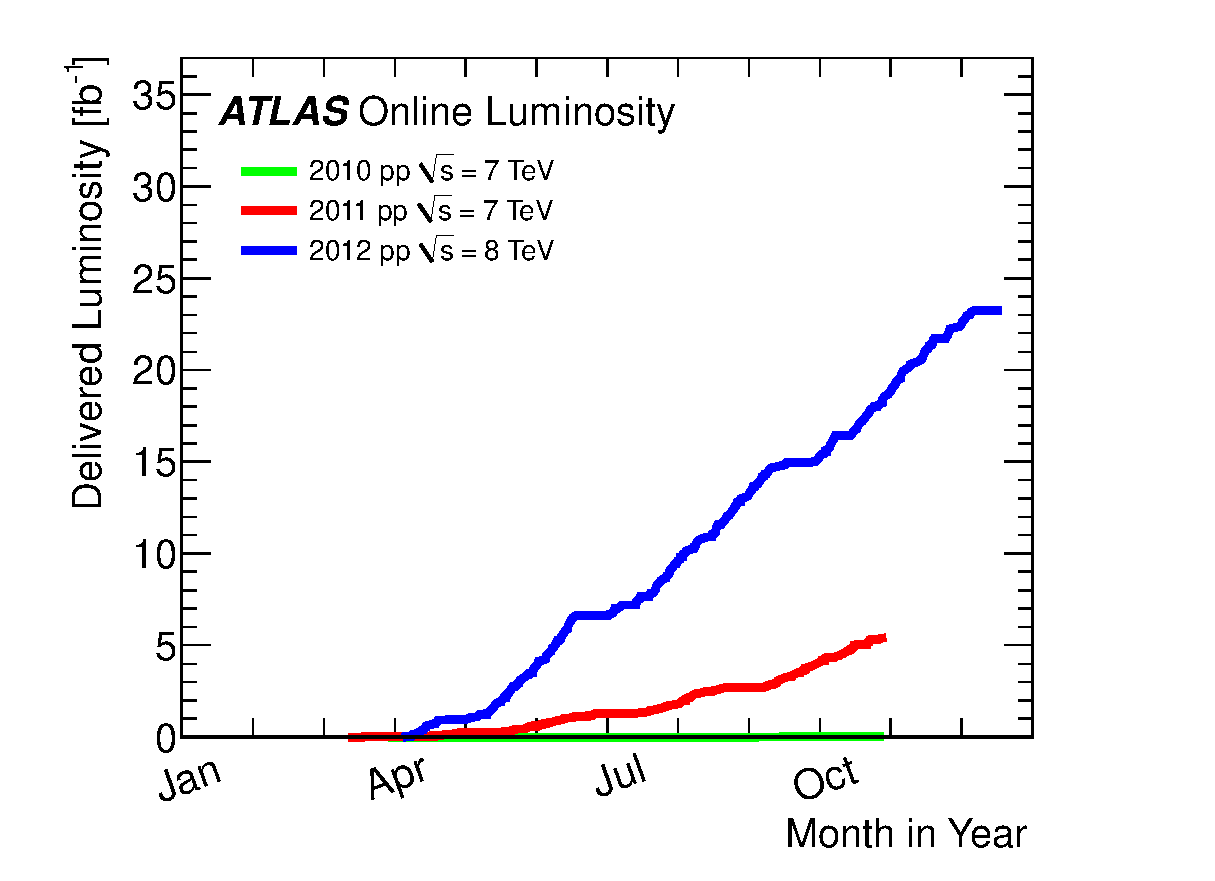
\includegraphics[width=0.48\textwidth]{figs/lhc/intlumivsyear.eps}
  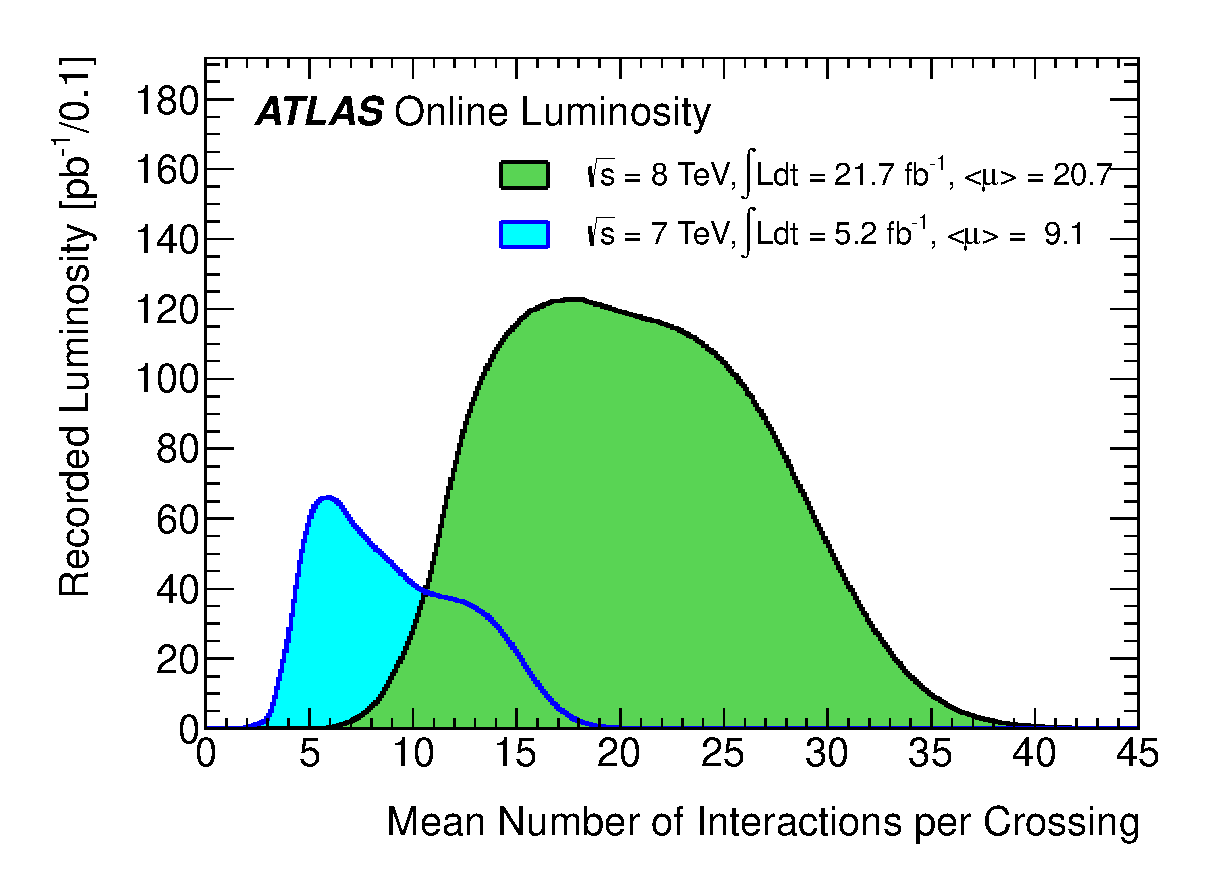
\includegraphics[width=0.48\textwidth]{figs/lhc/mu_2011_2012-dec.eps}
  \caption{
    (Left) Integrated luminosity of proton-proton collision data collected by
    ATLAS during the three years of Run 1.
    The rate of data collection was increased in part by increasing the number
    of interactions per crossing (right).
  }
  \label{fig:int_lumi_vs_time_and_pileup}
\end{figure}


%% ------------------------------------------------------------------------------
\FloatBarrier
\section{The \atlas\ experiment}

\begin{figure}[ht]
  \centering
  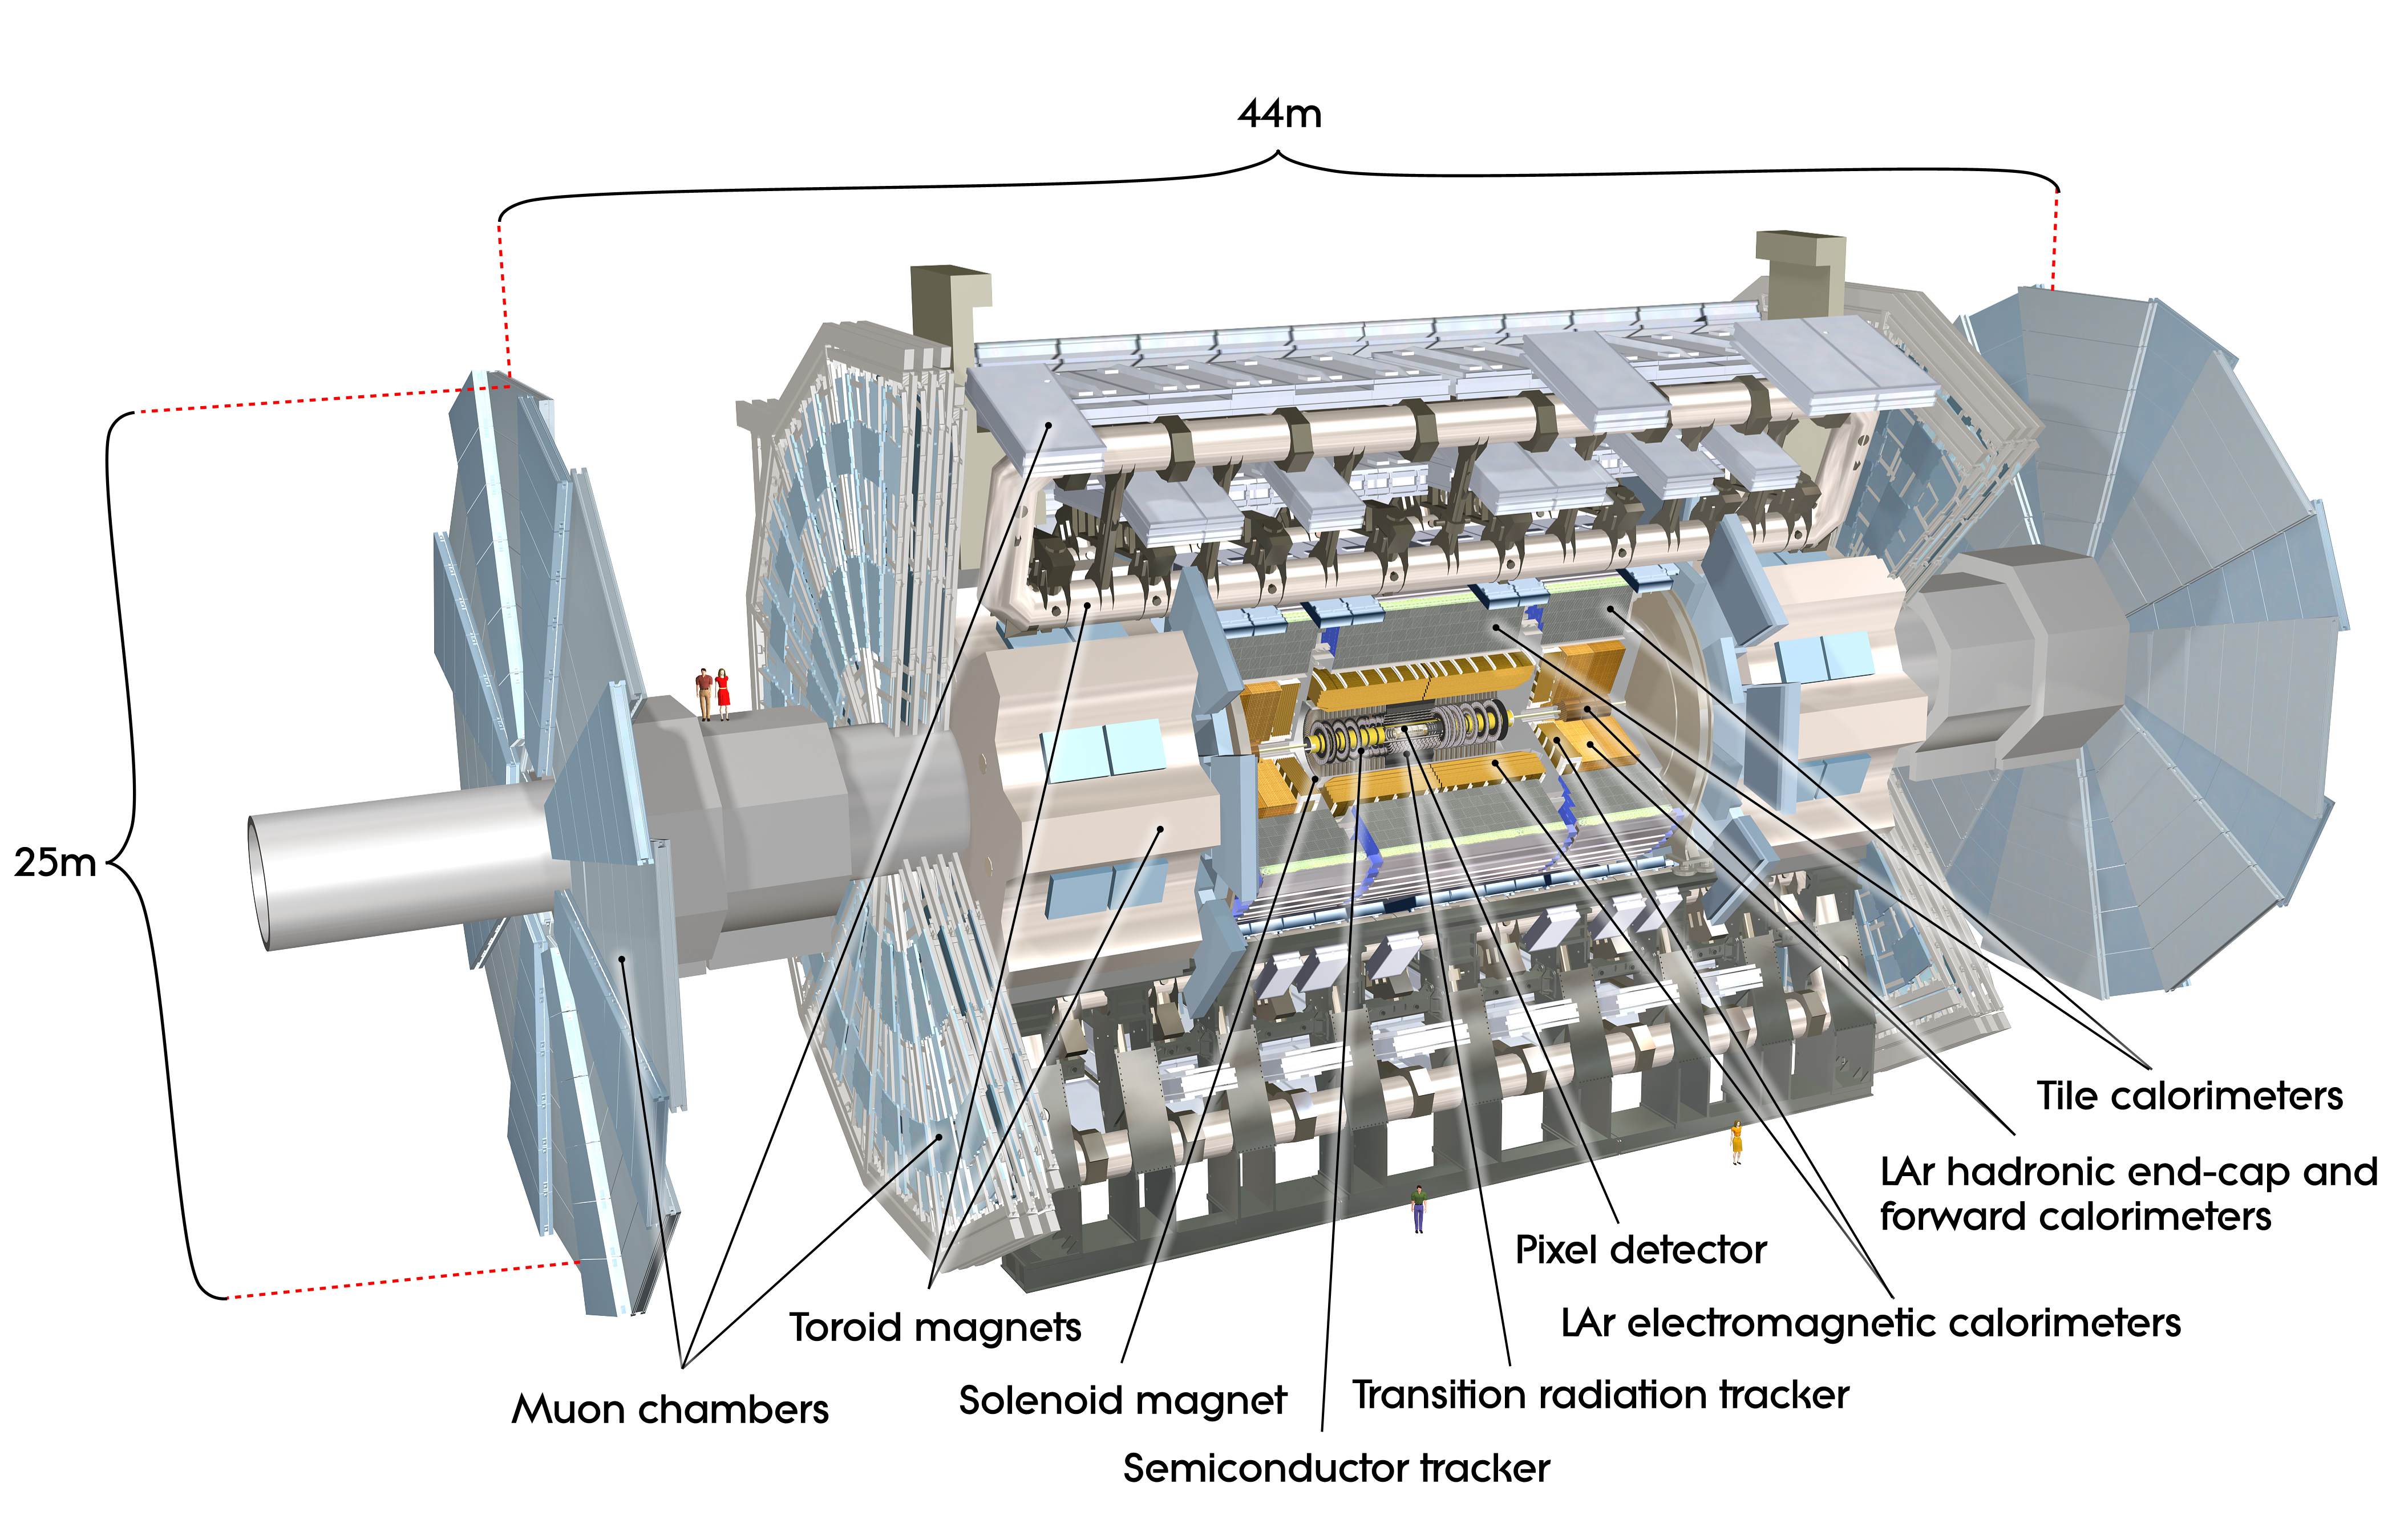
\includegraphics[width=\textwidth, clip=true, trim=0 0 0 0]
    {figs/lhc/atlas_det.jpg}
    % {figs/lhc/atlas_det_dino_1.jpg}
    % {figs/lhc/atlas_det_dino_2.jpg}
  \caption{
    The \atlas\ experiment~\cite{Pequenao:1095924}.
  }
  \label{fig:atlas_det}
\end{figure}

Along with \cms, \atlas\ is one of the two general purpose experiments, which
collect and analyze data from LHC collisions~\cite{cern-jinst-atlas}.
\atlas\ is located at interaction point 1 of the LHC, across the street from
the CERN Meyrin campus.
The experiment is made up of many ``sub-detectors,'' using an array of
technologies, which work together to reconstruct the collision events.
Figure~\ref{fig:atlas_det} shows a cut-away diagram of the ATLAS experiment,
highlighting the various sub-detectors.
Starting from the interaction point, and moving outward, the sub-detectors
are grouped into three main categories, an inner
detector~(Section~\ref{sec:id}), used to measure the trajectory of charged
particles, the calorimetry system~(Section~\ref{sec:calo}), which records the
energy deposition of particles, and a muon spectrometer~(Section~\ref{sec:ms})
which is used to identify and track muons.
These systems and their components are described in more detain in the coming
sections.

%% - - - - - - - - - - - - - - - - - - - - - - - - - - - - - - - - - - - - - - -
\FloatBarrier
\subsection{Coordinate system} 
\label{sec:coordinate_system}

\atlas\ uses a right-handed coordinate system with its origin at the nominal
interaction point (IP) in the center of the detector and the $z$-axis
along the beam pipe. The $x$-axis points from the IP to the center of the
LHC ring, and the $y$-axis points upward. Cylindrical coordinates
($R,\phi$) are used in the transverse plane, $\phi$ being the azimuthal
angle around the beam pipe. The pseudorapidity is defined in terms of the
polar $\theta$ angle as
\begin{equation}
  \eta = -\ln\left[\tan(\frac{\theta}{2})\right].
\end{equation}
The distance parameter (in $\eta$-$\phi$ space)
\begin{equation}
  \Delta R = \sqrt{(\Delta \eta)^2 + (\Delta \phi)^2}
\end{equation}
is used.

%% - - - - - - - - - - - - - - - - - - - - - - - - - - - - - - - - - - - - - - -
\FloatBarrier
\subsection{Inner detector} 
\label{sec:id}

\begin{figure}[p]
  \centering{
    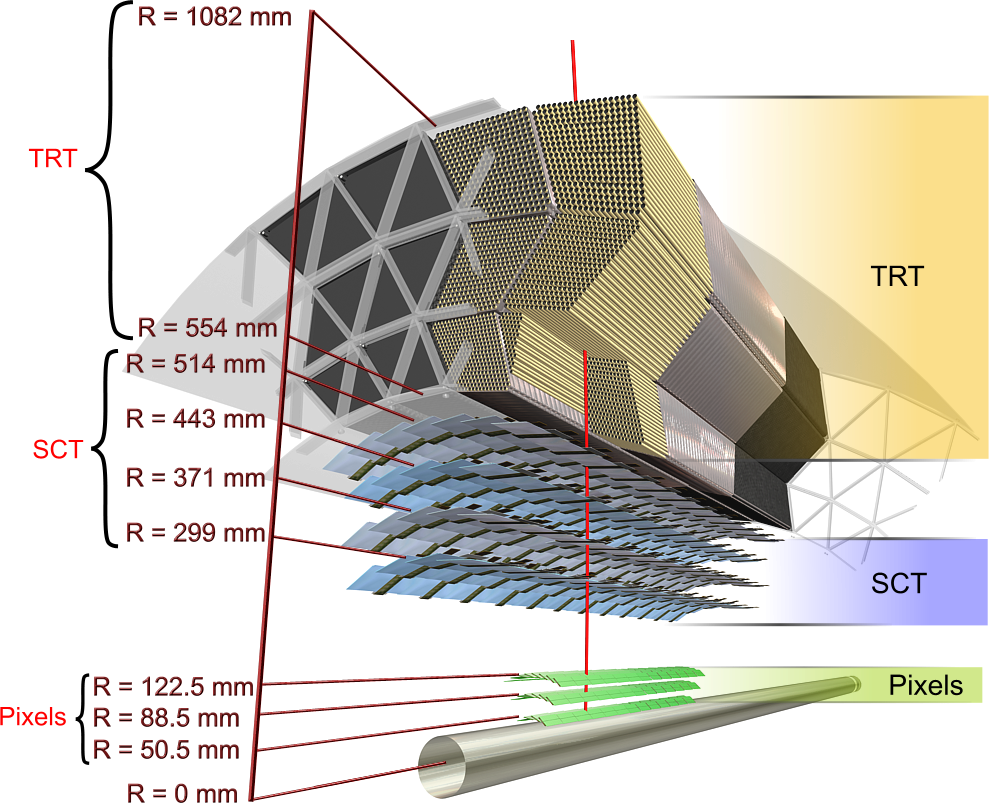
\includegraphics[width=0.8\textwidth]{figs/lhc/id_schematic_barrel.png}
    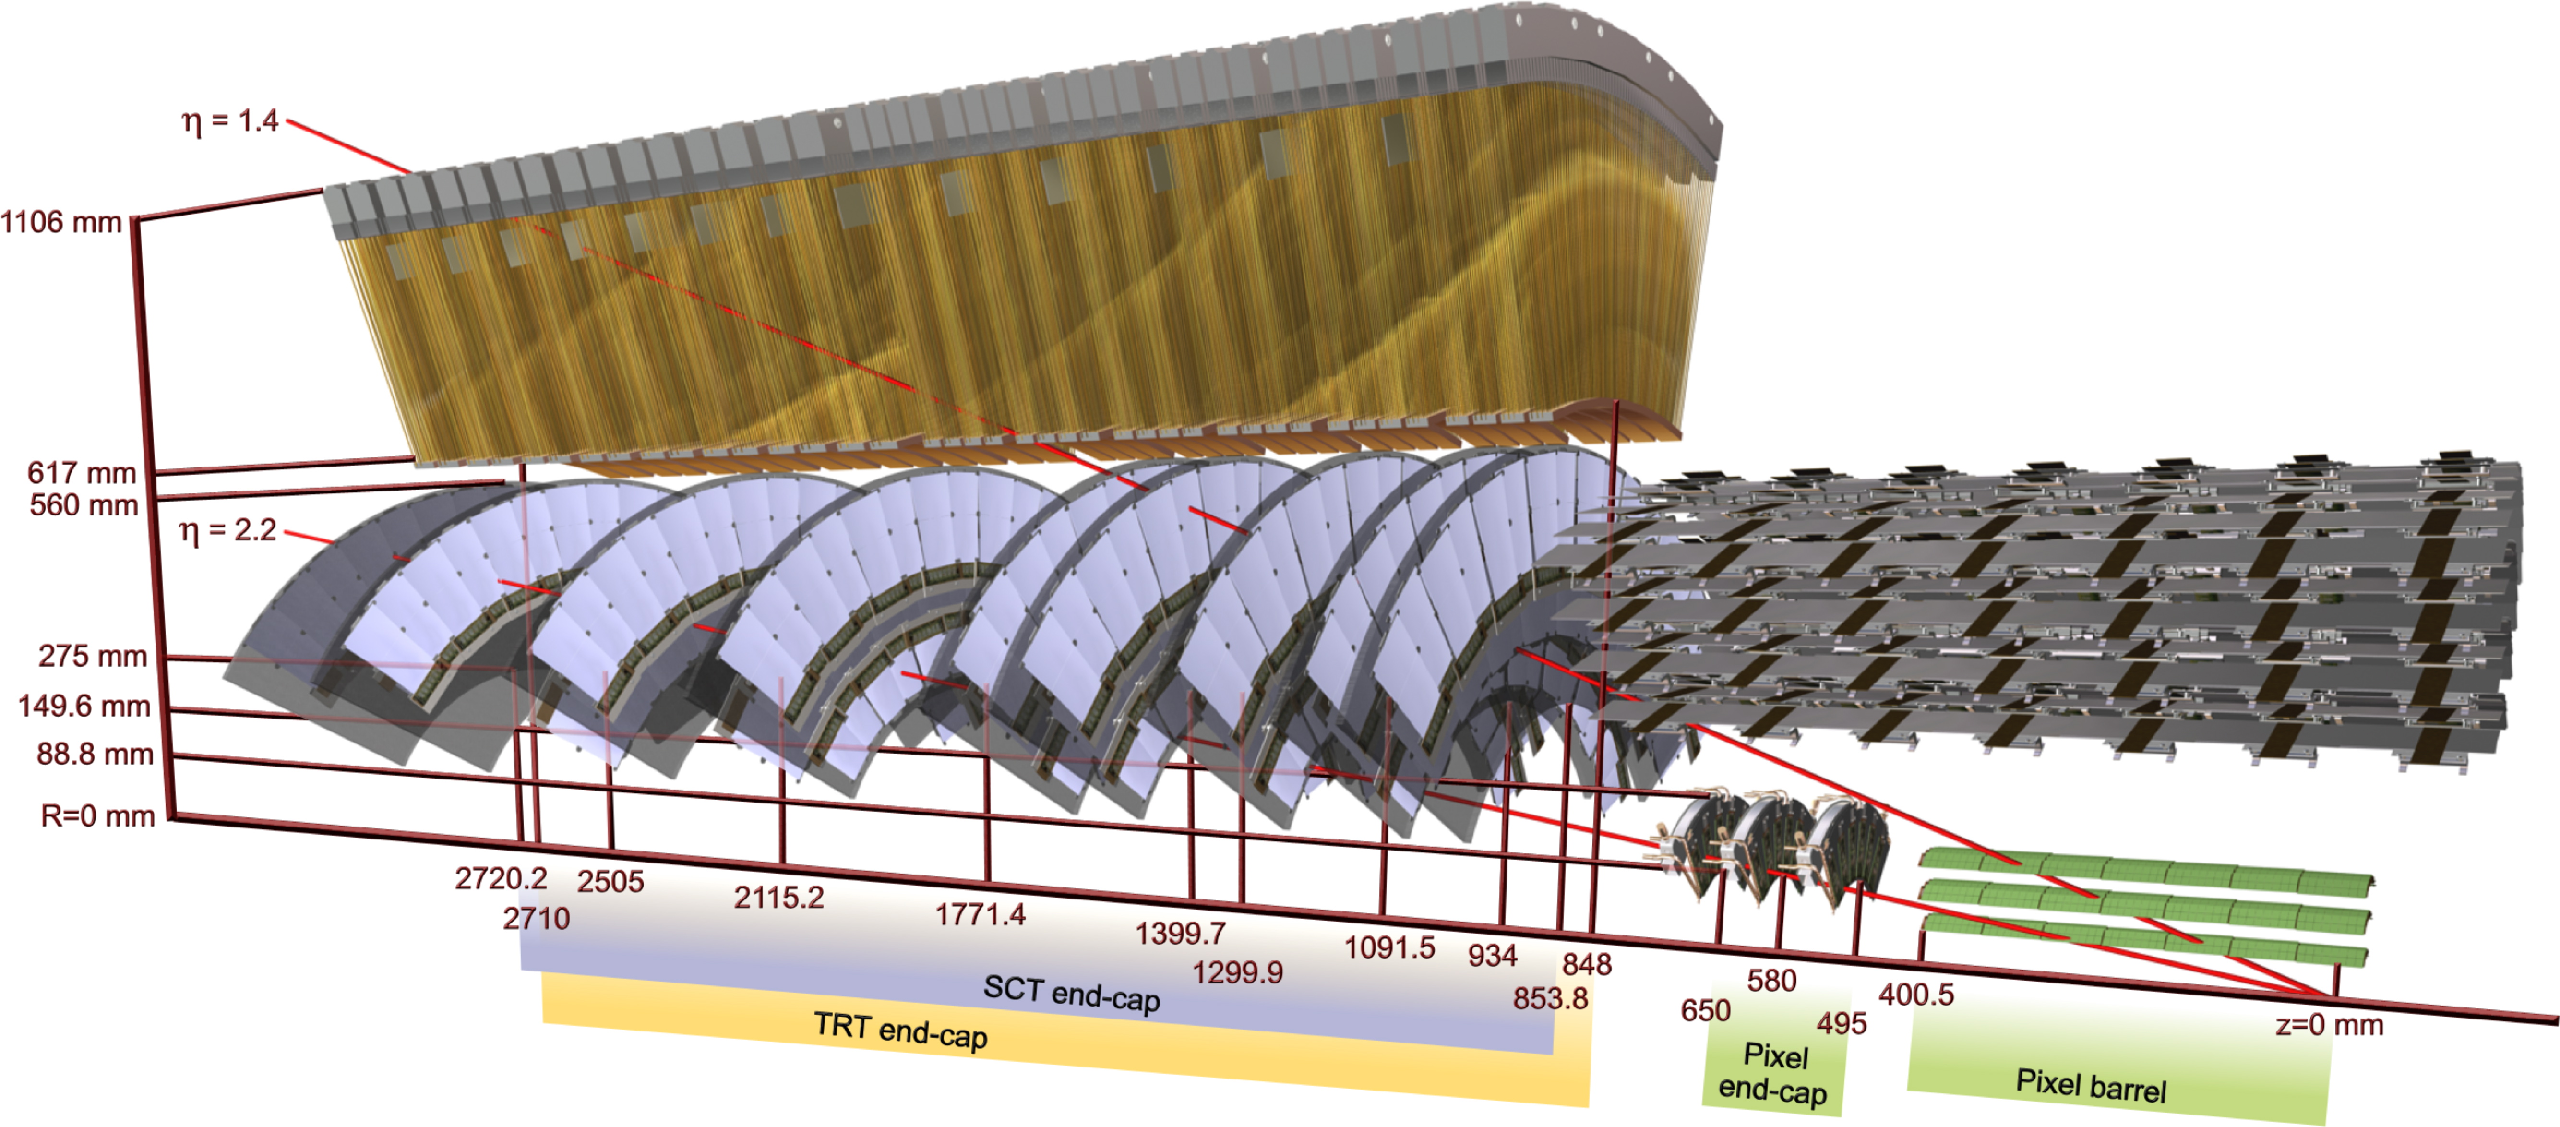
\includegraphics[width=0.9\textwidth]{figs/lhc/id_schematic_endcap.png}
  }
  \caption[
    Schematic of the inner detector of the
    \atlas\ experiment~\cite{1748-0221-3-08-S08003}.
  ]{
    Schematic of the inner detector of the \atlas\ experiment.
    The barrel (top) and endcap (bottom) are show separately.
    The inner detector is made up of layers, consisting of the silicon pixels,
    the silicon semiconductor tracker (SCT), and the transition radiation
    tracker (TRT)~\cite{1748-0221-3-08-S08003}.
  }
  \label{fig:id_cartoon}
\end{figure}

The inner detector (ID) makes up the three innermost sub-detectors of ATLAS,
the pixel detector, silicon semiconductor tracker (SCT), and the transition
radiation tracker (TRT), shown in Figure~\ref{fig:id_cartoon}.
All three sub-detectors of the ID work together to reconstruct the trajectory
of charged particles from collision events.
The pixel and SCT detectors use silicon technologies, while he TRT employs
straws filled with a Xenon gas mixture.
The three sub-detectors are described in \Cref{sec:pixel,sec:sct,sec:trt},
and tracking is reviewed in Section~\ref{sec:tracking}.

%% - - - - - - - - - - - - - - - - - - - - - - - - - - - - - - - - - - - - - - -
\FloatBarrier
\subsubsection{Pixel detector} 
\label{sec:pixel}

\begin{figure}[ht]
  \centering{
    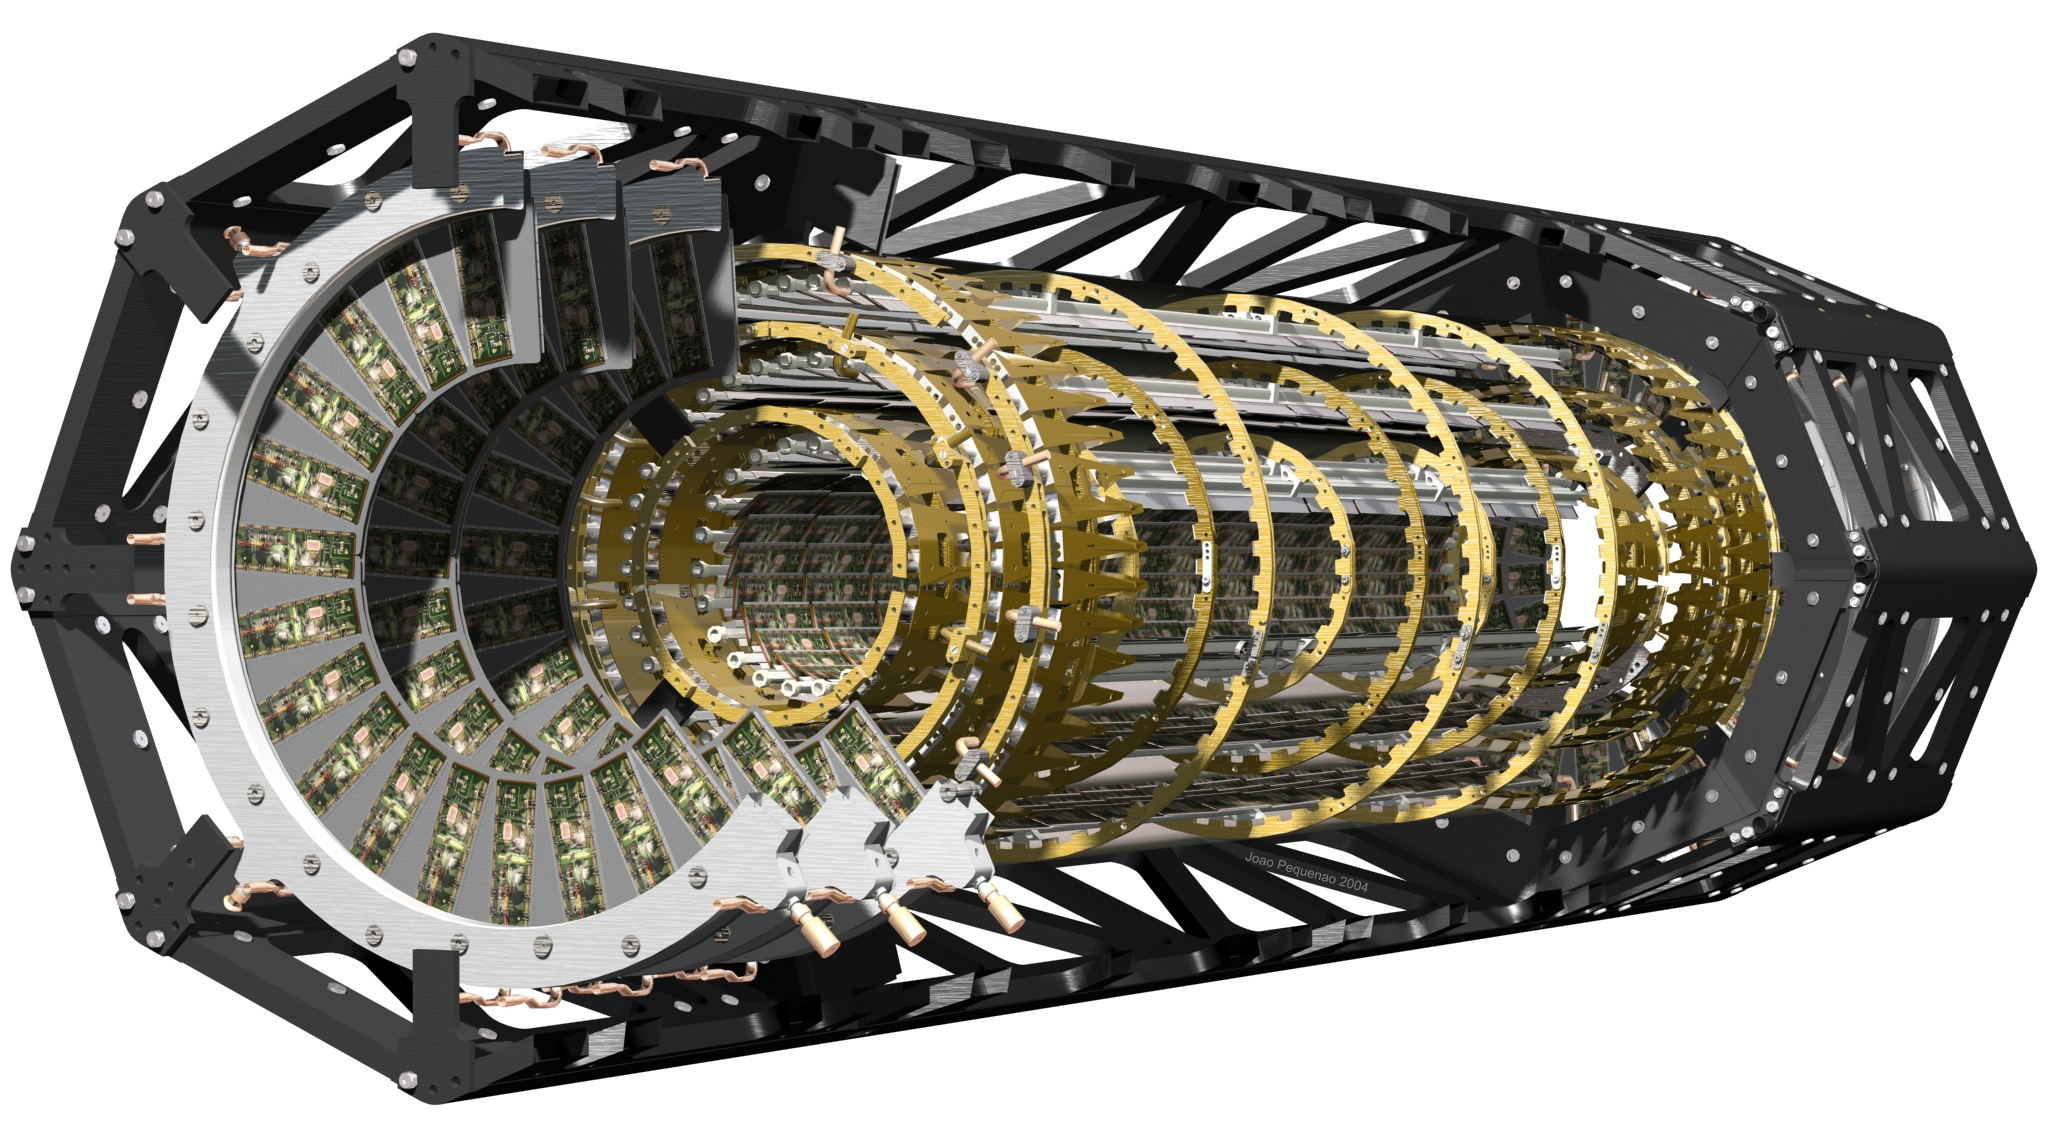
\includegraphics[width=\textwidth]{figs/lhc/pixel_schematic.jpg}
  }
  \caption{
    The Silicon pixel tracker of the \atlas\ experiment~\cite{Pequenao:1095925}.
  }
  \label{fig:pixel_cartoon}
\end{figure}

% \begin{figure}[ht]
%   \centering{
%     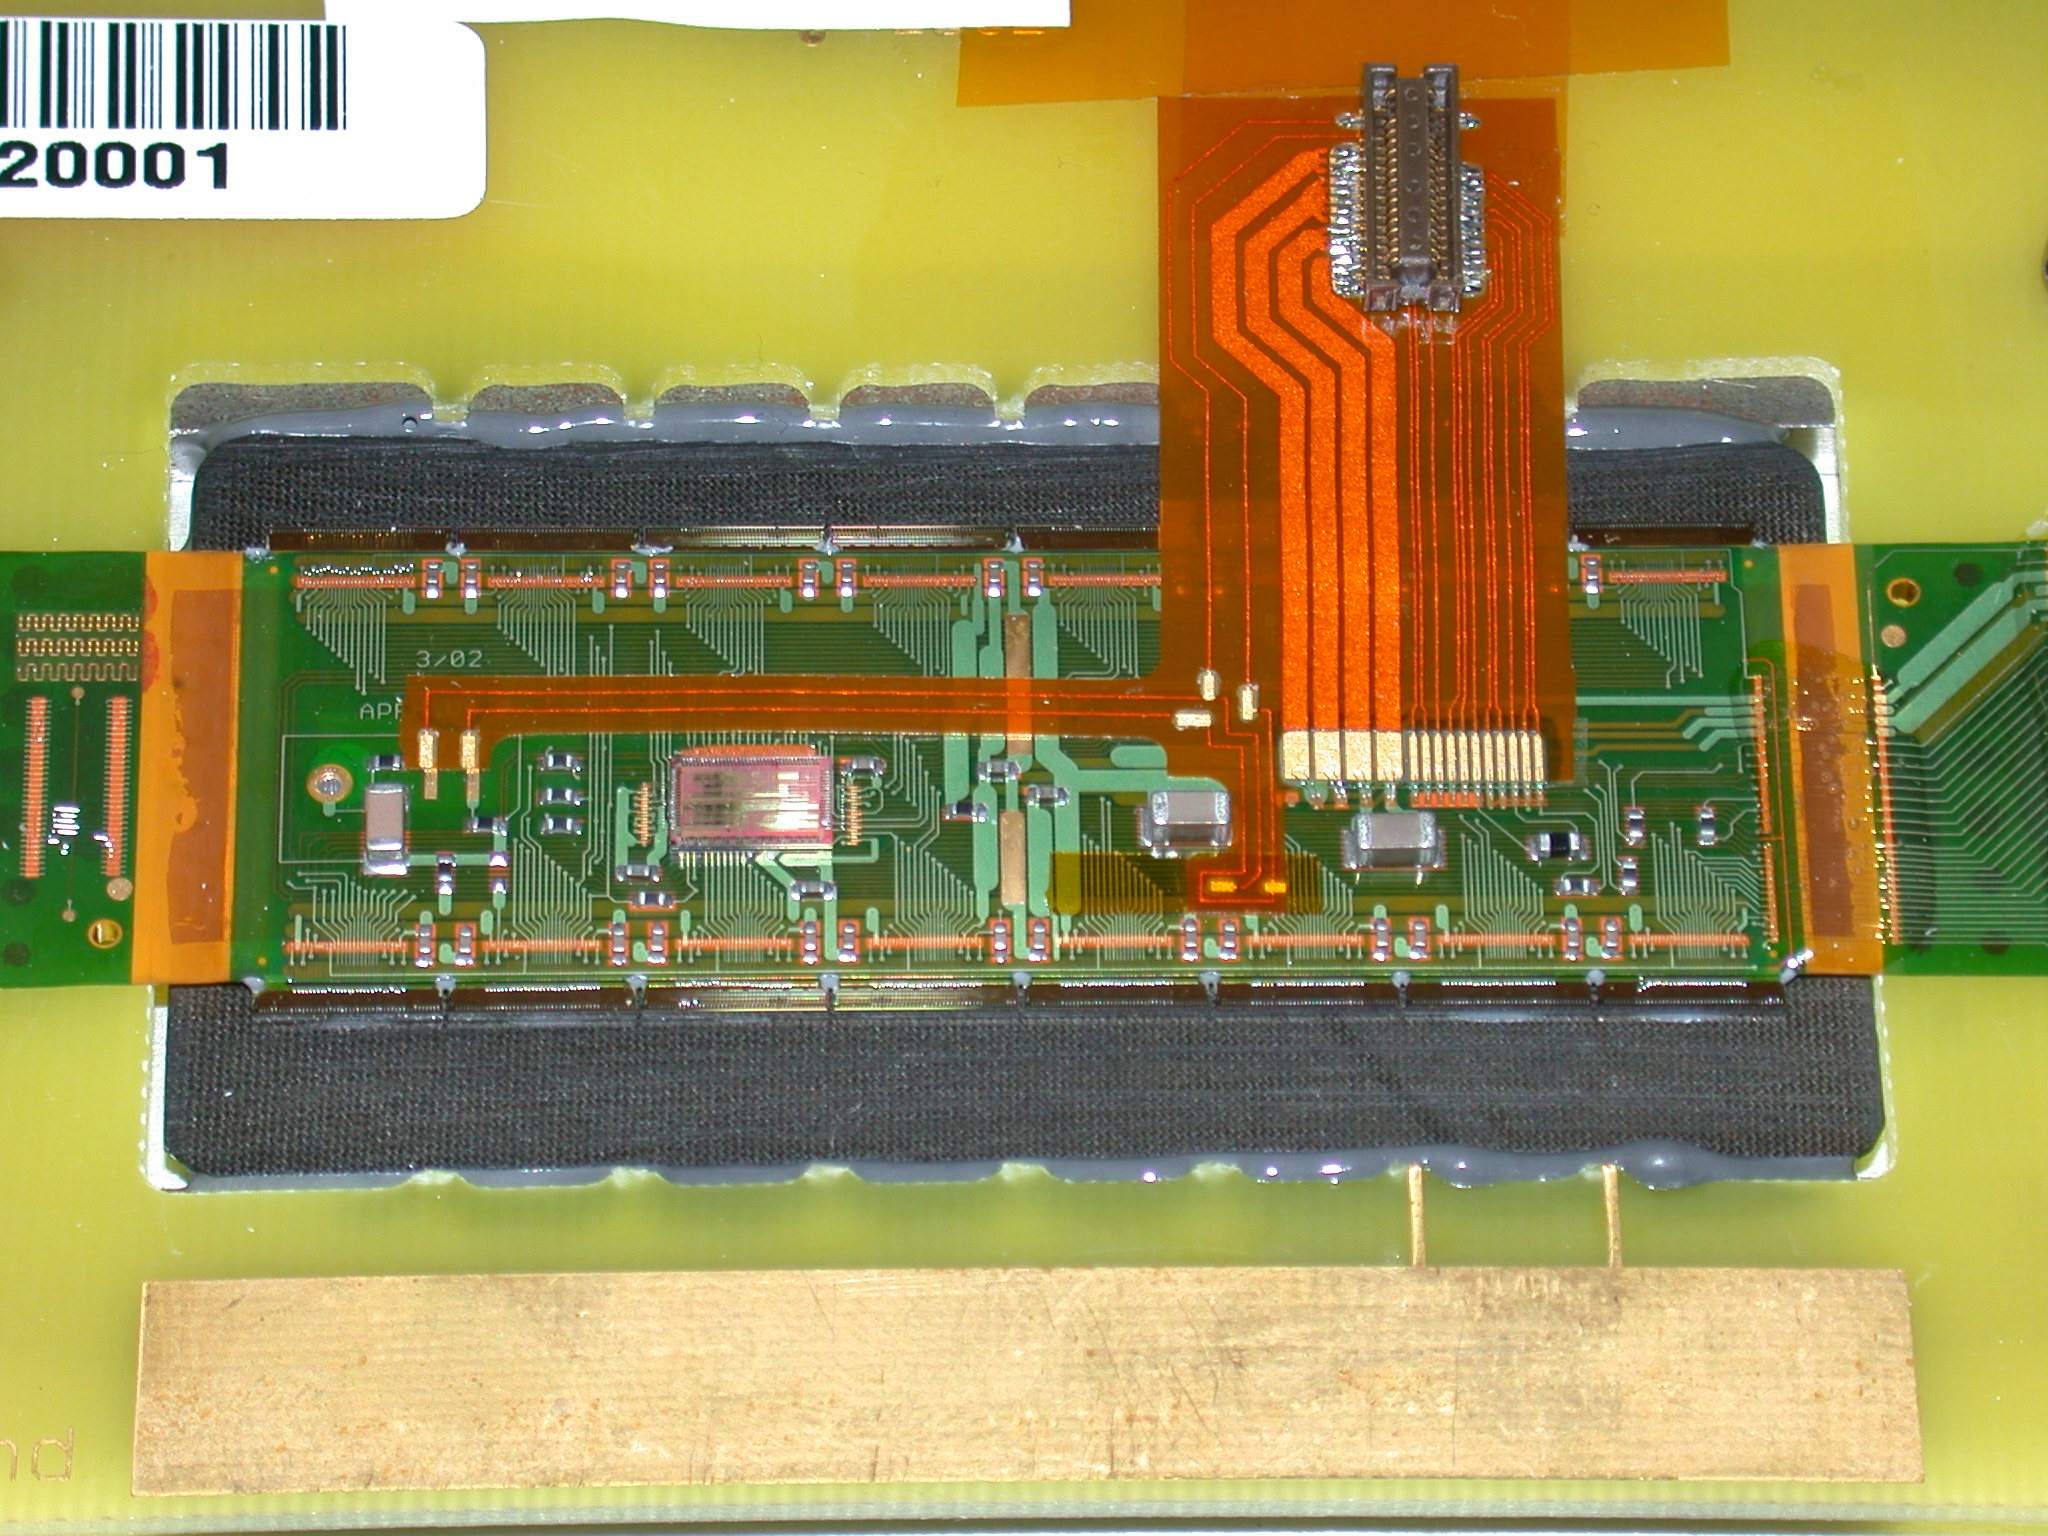
\includegraphics[width=0.8\textwidth]{figs/lhc/pixel_module.jpg}
%   }
%   \caption{{\color{red}TODO}~\cite{Wermes:43561}.}
%   \label{fig:pixel_module}
% \end{figure}

The pixel detector, shown in Figure~\ref{fig:pixel_cartoon}, is the closest
sub-detector in \atlas\ to the interaction point.
It uses silicon pixel technology to provide high granularity for precision
tracking.
The detector consists of three barrel layers, at radii of 50.5~mm, 88.5~mm,
and 122.5~mm, and three disks on either side of the barrel, with mean $z$-values
of 495~mm, 580~mm, and 650~mm.
The pixel detector provides coverage up to $|\eta| = 2.5$.
In total, there are $80 \times 10^{6}$ channels in the pixel detector, each 
with a nominal pixel size is 50~\um\ in the $\phi$ dimension, and 400~\um\ in
$z$~\cite{1748-0221-3-07-P07007}.

%% - - - - - - - - - - - - - - - - - - - - - - - - - - - - - - - - - - - - - - -
\FloatBarrier
\subsubsection{Silicon semiconductor tracker} 
\label{sec:sct}

\begin{figure}[ht]
  \centering{
    \includegraphics[width=\textwidth]{figs/lhc/sct_photo.jpg}
  }
  \caption{
    Photograph of the silicon semiconductor tracker of the
    \atlas\ experiment~\cite{Maximilien:883305}.
  }
  \label{fig:sct_photo}
\end{figure}

% \begin{figure}[ht]
%   \centering{
%     \includegraphics[width=0.8\textwidth]{figs/lhc/sct_close_up.jpg}
%   }
%   \caption{{\color{red}TODO}~\cite{Maximilien:43814}.}
%   \label{fig:sct_close_up}
% \end{figure}

The SCT, shown in Figure~\ref{fig:sct_photo}, is also made of silicon
detectors, but rather than pixels, the SCT uses microstrip technology.
The detector is made up of four double layers in the barrel, and nine
endcap layers on each side of the barrel.
The SCT provides coverage up to $|\eta| = 2.5$.
A charged particle has, on average, eight hits in the SCT, with each hit
in the barrel (endcap) having a resolution of 17~\um\ in the
$r-\phi$~($z-\phi$)~plane, and 580~\um\ in the $z$ ($r$) dimension.
There are 6.3 million read-out channels in the SCT.

%% - - - - - - - - - - - - - - - - - - - - - - - - - - - - - - - - - - - - - - -
\FloatBarrier
\subsubsection{Transition radiation tracker} 
\label{sec:trt}

\begin{figure}[ht]
  \centering{
    \includegraphics[width=\textwidth]{figs/lhc/trt_photo.jpg}
  }
  \caption{
    Photograph of the transition radiation tracker of the
    \atlas\ experiment during its commissioning~\cite{Maximilien:889555}.
  }
  \label{fig:trt_module}
\end{figure}

The TRT, shown during the commissioning process in Figure~\ref{fig:trt_module}
makes up the largest and outer layer of the ID, and is used for both tracking
and particle identification.
The TRT covers provides coverage up to $|\eta| - 2.0$.
The TRT employs 350,000 straws filled with a gas mixture made up of
Xe~(70\%), $\text{CO}_2$~(27\%), and $\text{O}_2$~(3\%).
Each straw of the TRT has a 4~mm diameter, and is strung with a gold plated
tungsten alloy wire.
The outer wall of the straws is at a high electric potential, inducing a large
electric field inside the straw.
Charged particles pass through the straw, ionizing the electric field,
resulting is a charge deposition on the wire, and a measurable current.

The TRT has a less precise resolution than the silicon trackers, but a charged
particle track may have more than 30 TRT hits, which can be combined to make
up for for some of the difference in precision.
The TRT barrel has a precision of 130~\um\  in the $r-\phi$ plane, but much
worse resolution $z$ since there is little segmentation in this dimension.

The TRT is also designed for use in particle identification.
Transition radiation (TR) is emitted when a charged particle crosses a boundary
between media with different dielectric constants.
The amount of TR is proportional to the Lorentz~$\gamma$ factor, which is in
turn related to the particle mass.
Electrons are roughly 200 times less massive than pions, so have a higher
probability to emit TR while crossing a boundary.
The space between the TRT straws is filled with radiator material providing
many such boundaries to facilitate TR.
Xe was chosen as the active gas because it has a large absorption cross section
for TR photons.
The absorption of the additional TR photons induces more ionization, and
therefore, more charge to build up on the wire.
All this results in a larger signal, which can be detected by the TRT
front-end electronics.
The TRT operates with two threshold values (low- and high-threshold).
The low threshold is used for tracking, and is tuned for the typical amount of
ionization from a charged particle passing through the TRT straws.
The high threshold is tuned to register the larger signal when the Xe gas
absorbs the TR photons.
The fraction of TRT hits associated with a charged particle track that exceed
the high threshold is a discriminating variable used to identify electrons.

%% - - - - - - - - - - - - - - - - - - - - - - - - - - - - - - - - - - - - - - -
\FloatBarrier
\subsubsection{Tracking} 
\label{sec:tracking}

The ID is used to reconstruct the trajectory of charged particles.
The individual measurements made along the trajectory of the charged particle
are referred to as ``hits.''
Hits from the three ID sub-detectors are combined into tracks using Kalman
filtering tools which account for multiple scattering as a particle traverses
the ID~\cite{ATLAS-CONF-2014-047,ATLAS-CONF-2012-042}.

The ID is enclosed inside a solenoid magnet, with a field strength of 2~T.
The magnetic field bends the trajectory of moving charged particles
perpendicular to the field direction according to
$\vec{F} = q \vec{v}\times \vec{B}$.
The magnetic field is pointing along the direction of the beam, so charged
particles coming from the interaction point will form a helix, with radius
of curvature determined by the transverse momentum (\pt).
Particles with low \pt\ will bend more than those with higher \pt.
The \pt\ of charged particle tracks is determined based on the measured radius
of curvature.
\begin{equation}
  \pt = qBr_\mathrm{curvature}
\end{equation}
It should be noted that the charge is not directly measured, but the sign of
the charge is determined based on the direction the particle is bent.
The momentum resolution of the tracking is limited by the position resolution.
As the tracks become more straight, the precision of curvature becomes worse,
resulting in worse momentum resolution for these high-\pt\ tracks.
The relative momentum resolution is proportional to the \pt\ of the that track.

%% - - - - - - - - - - - - - - - - - - - - - - - - - - - - - - - - - - - - - - -
\FloatBarrier
\subsection{Calorimetry} 
\label{sec:calo}

\begin{figure}[ht]
  \centering{
    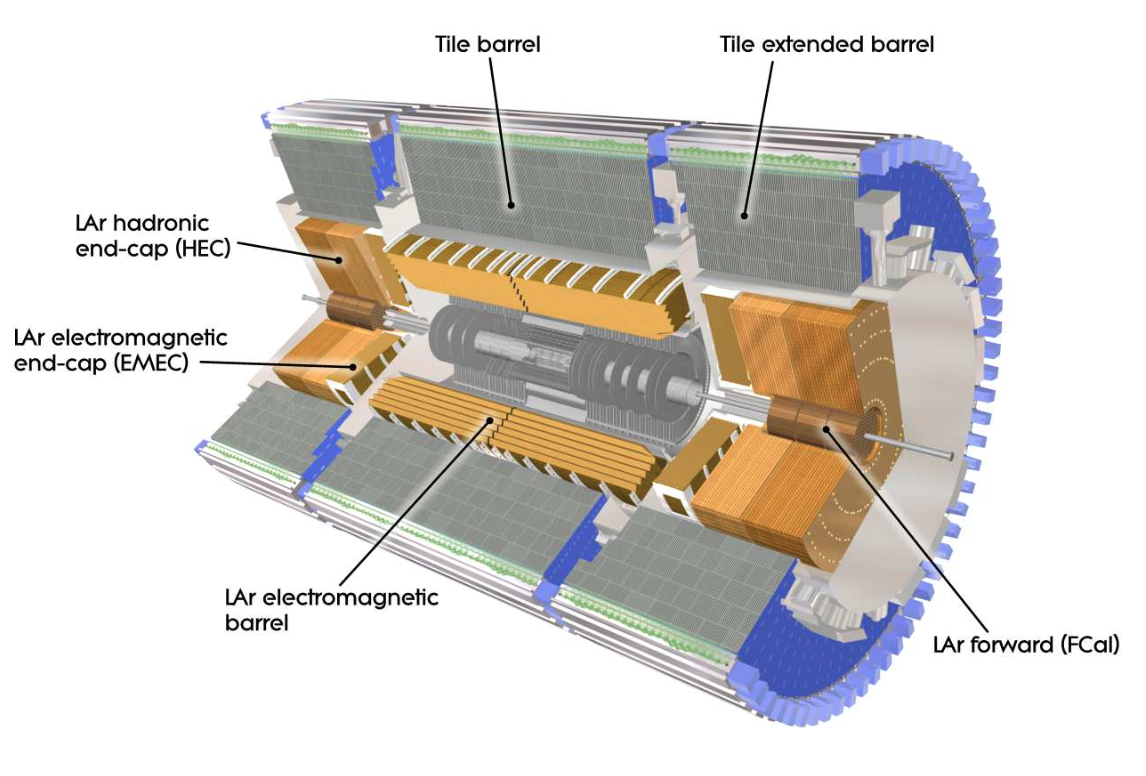
\includegraphics[width=\textwidth]{figs/lhc/calo_schematic.png}
  }
  \caption[
    Schematic of the calorimeter system of the
    \atlas\ experiment~\cite{cern-jinst-atlas}.
  ]{
    Schematic of the calorimeter system of the
    \atlas\ experiment.
    The calorimetry system is comprises the electromagnetic calorimeter,
    and a hadronic calorimeter~\cite{cern-jinst-atlas}.
  }
  \label{fig:calo_cartoon}
\end{figure}

The calorimetry system, situated outside the ID and the solenoid, is shown
in Figure~\ref{fig:calo_cartoon}.
The calorimetry systems of \atlas\ are designed to compliment one another and
offer full coverage in the $\phi$, and pseudorapidity coverage up to
$|\eta| = 4.9$.
The objective of the calorimeters is to stop particles like electrons, photons,
and hadrons and measure their energy.
\atlas\ uses ``sampling calorimeters,'' which absorb a fraction of the total
energy, and must infer the full shower energy.
This is achieved using a dense absorber material to initial a shower, and
an active material to sample the energy deposition.

The calorimetry system is broken up into three sub-systems, the electromagnetic
calorimeter (EM calorimeter), the hadronic calorimeter, and the forward
calorimeter (FCal).
Each of the sub-systems employ different absorber and active materials.

Unlike tracking systems, like the ID, the energy resolution from a calorimeter
actually improves with higher energy deposition.

%% - - - - - - - - - - - - - - - - - - - - - - - - - - - - - - - - - - - - - - -
\FloatBarrier
\subsubsection{Electromagnetic calorimeter} 
\label{sec:ecal}

The EM calorimeter is used to stop and measure the energy of electrons and
photons.
It is broken into a barrel component, covering $|\eta| < 1.5$, and two endcaps,
covering $1.4 < |\eta| < 3.2$.
Lead plates are used as an absorber material, and the active material is
liquid argon (LAr).
A pre-sampler is installed in the region $|\eta| < 1.8$ to sample energy from
showers initiated before the first absorber plate.

The active material is arranged in an accordion-style geometry to ensure full
coverage in $\phi$.
The barrel region is further sub-divided into three layers, with differing
granularity.
The first layer has the finest granularity, being arranged in strip-shaped
cells with $\Delta\eta \times \Delta\phi = 0.025/8 \times 0.1$.
This level of granularity provides good position resolution, which is useful
in particle identification.
The second layer is arranged in square cells, measuring
$\Delta\eta \times \Delta\phi = 0.025 \times 0.025$.
Layer 2 is the thickest layer, with 16 radiation lengths.
The third layer is coarser than the previous
layers~($\Delta\eta \times \Delta\phi = 0.050 \times 0.025$), and is used to
capture any remaining energy from the electromagnetic shower.

%% - - - - - - - - - - - - - - - - - - - - - - - - - - - - - - - - - - - - - - -
\FloatBarrier
\subsubsection{Hadronic calorimeter} 
\label{sec:hcal}

The hadronic calorimeter is also broken up into barrel and endcap sections, but
in this case, the two regions use different materials.
The barrel section covers a region with $|\eta| < 1.7$, and uses steel
absorbers and scintillating tiles as an active material.
The endcaps use copper plates as an absorber material, and LAr for the active
material.
The hadronic calorimeter endcaps span $1.5 < |\eta| < 3.2$.
Since the hadronic calorimeter is not used in particle identification, it is
much coarser than the EM calorimeter, with granularity
$\Delta\eta \times \Delta\phi = 0.1 \times 0.1$.

%% - - - - - - - - - - - - - - - - - - - - - - - - - - - - - - - - - - - - - - -
\FloatBarrier
\subsubsection{Forward calorimeter} 
\label{sec:fcal}

The FCal captures energy from particles in the very forward region
($3.1 < |\eta| < 4.9$).
It is made up of three layers in each endcap, each using LAr as the active
material.
The first layer uses coper absorber, while the second and third layers utilize
as an tungsten absorption material.

%% - - - - - - - - - - - - - - - - - - - - - - - - - - - - - - - - - - - - - - -
\FloatBarrier
\subsection{Muon spectrometer} 
\label{sec:ms}

\begin{figure}[ht]
  \centering{
    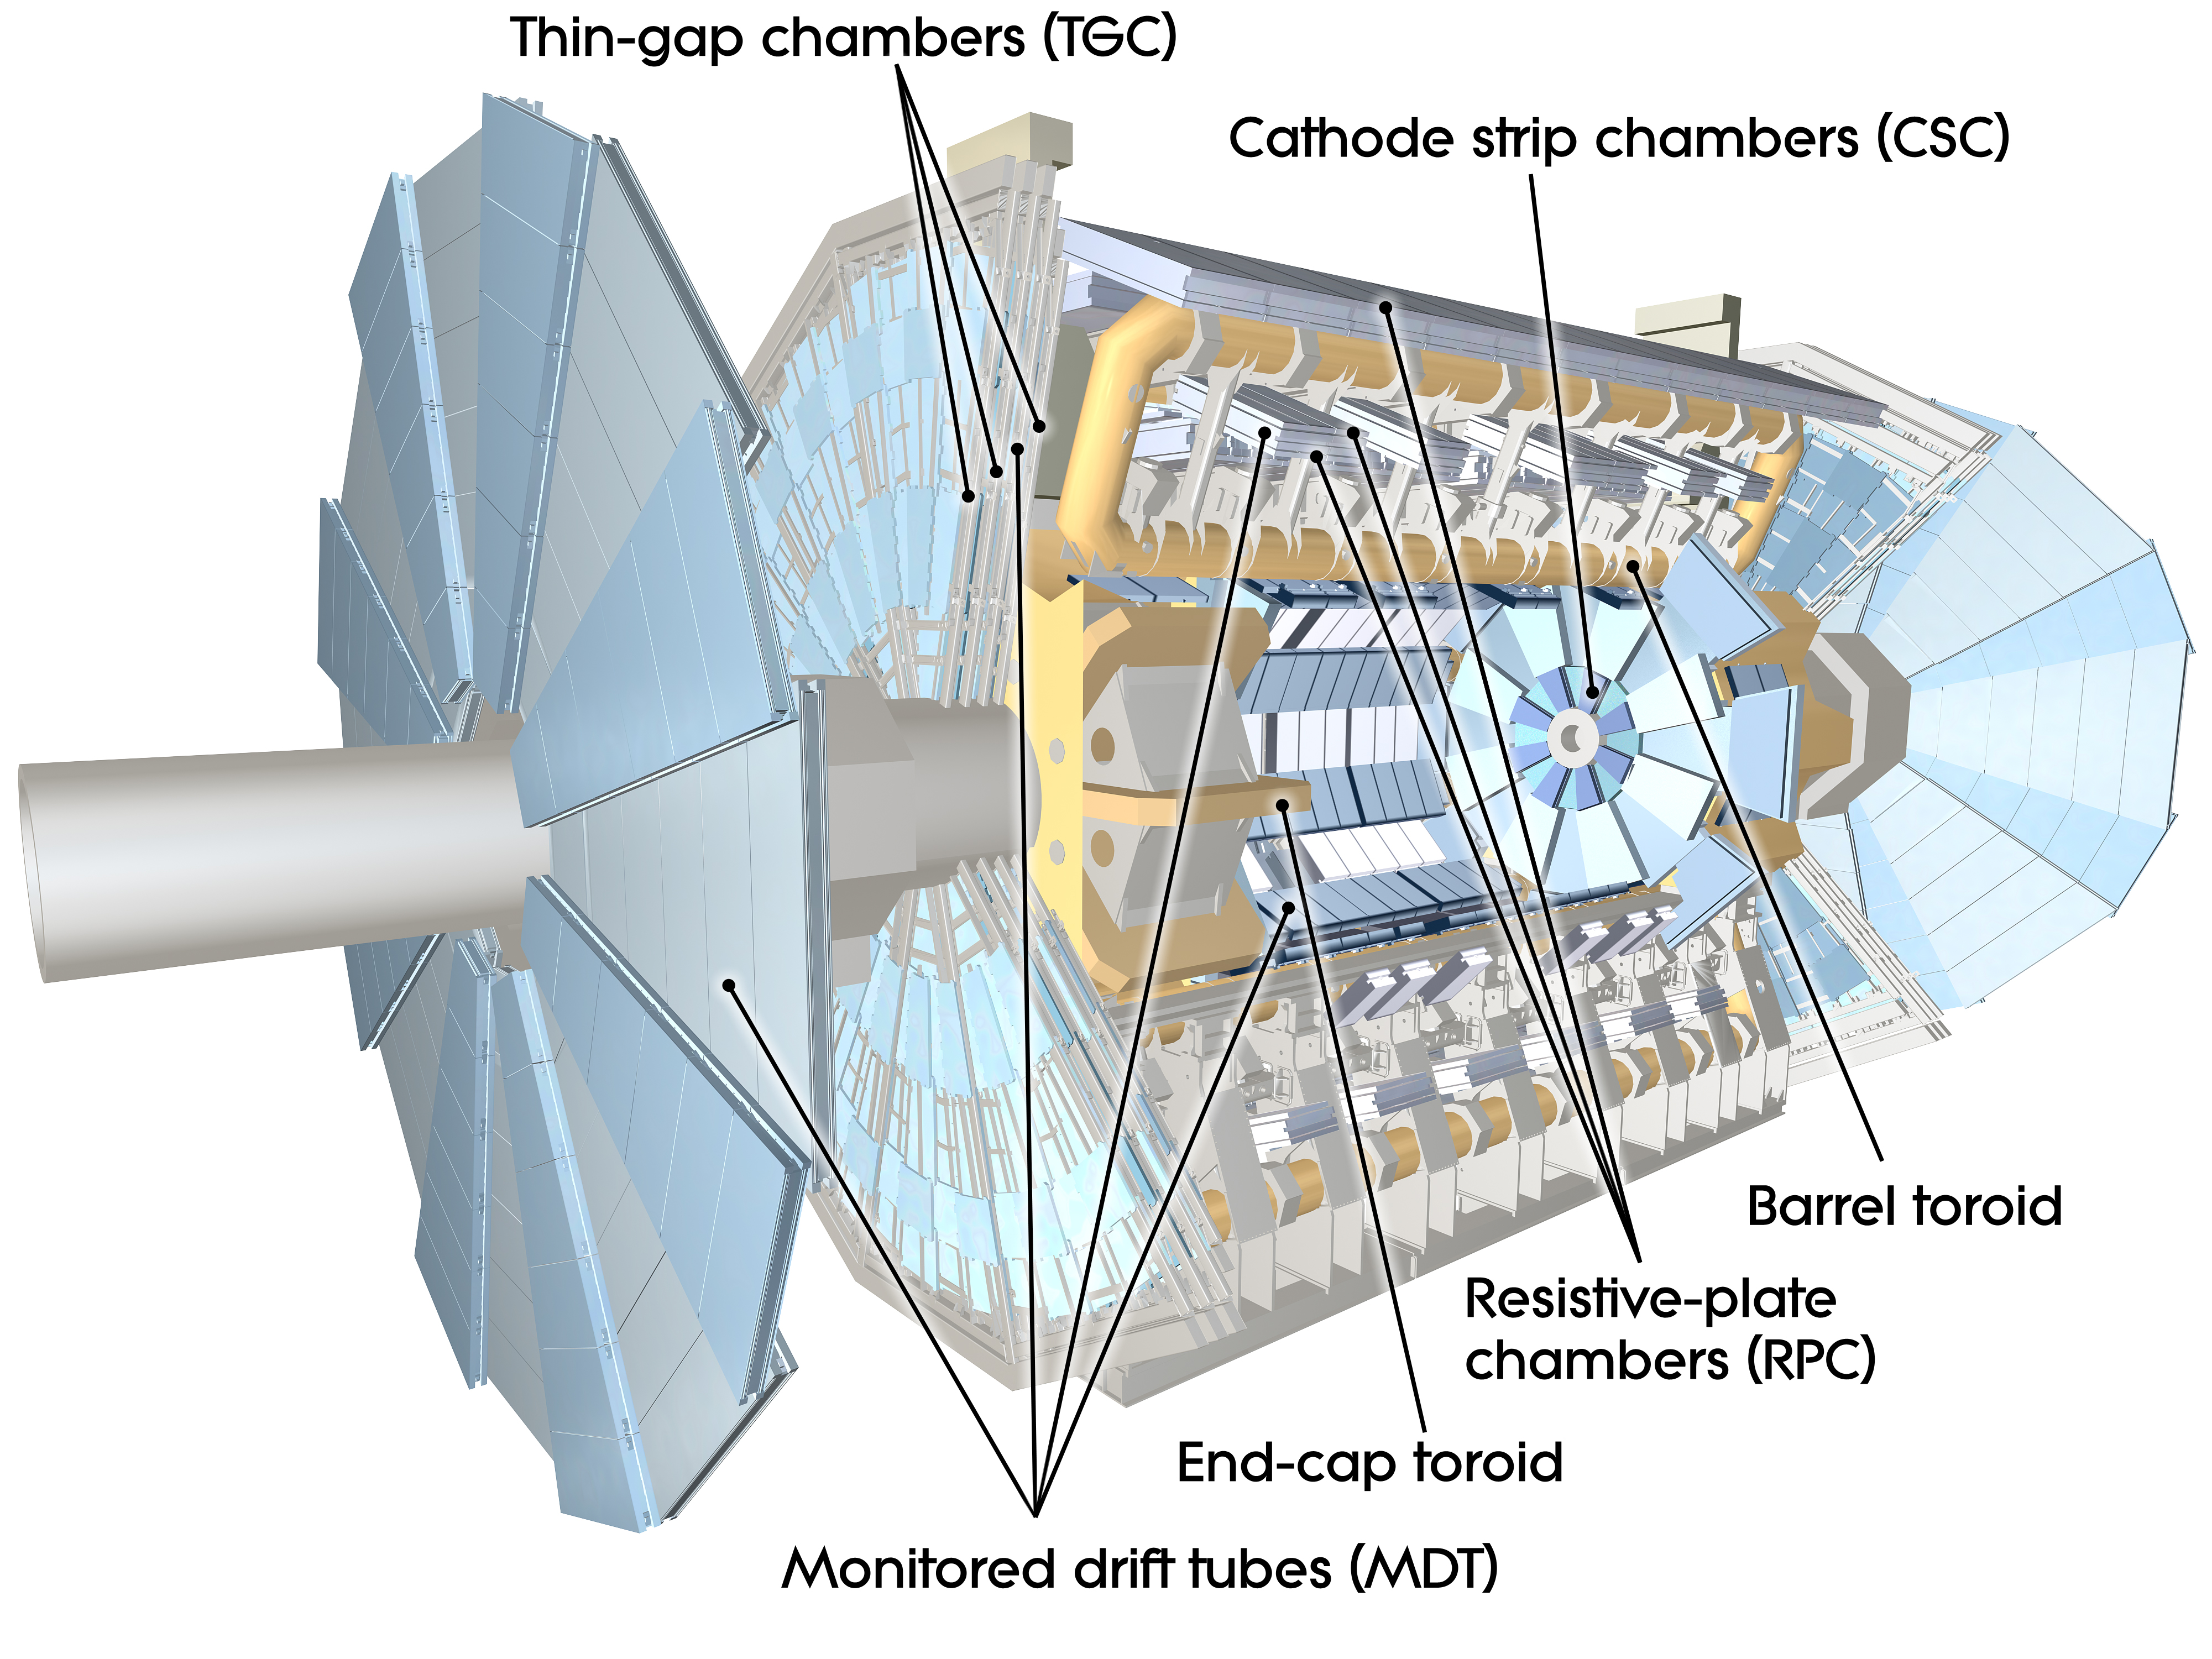
\includegraphics[width=\textwidth]{figs/lhc/ms_schematic.jpg}
  }
  \caption{
    Schematic of the muon systems of the
    \atlas\ experiment~\cite{Pequenao:1095929}.
  }
  \label{fig:ms_cartoon}
\end{figure}

The muon spectrometer (MS) comprise the four sub-detectors of the
\atlas\ experiment furthest from the interaction point, and is shown in
Figure~\ref{fig:ms_cartoon}.
Muons are minimum ionizing particle, and if they have sufficient energy, are
able to pass through the calorimetry system unstopped.
The MS has coverage up to $|\eta| = 2.7$, and is designed to make precision
tracking measurements of the muon trajectory and momentum.
A strong magnetic field is generated by eight large toroidal magnets in the
barrel, and two endcap toroid systems.
The magnetic field is situated such that the muons bend in the $\eta$
direction.
The four sub-detectors of the MS are
\begin{description}
  \item[Monitored drift tubes (MDTs):] 
    Approximately 370,000 drift tubes, each with diameter of 30~mm, and made of
    aluminum with a wire in the middle.
    The gas in the tube is ionized in the presence of a muon, and attracted to
    the wire in the center of the tube, leading to a measurable signal, which
    is read out by the electronics.
    The MDTs span the full range of the MS system ($|\eta| < 2.7$).
  \item[Cathode strip chambers (CSCs):] 
    Chambers, consisting anode wires and cathode strips.
    As a muon passes through a CSC, the gas within the chamber is ionized, and
    drifts toward the cathode strips, where the signal is read out.
    The relative size of the signal on adjacent strips is used to determine the
    location of the hit.
    The CSCs are located closer to the interaction point than the MDTs, in the
    region $2.0 < |\eta| < 2.7$.
  \item[Resistive plate chambers (RPCs):] 
    Consist of two resistive plates with a small gap, filled with gas.
    The gas is ionized in the presence of a muon, and drifts toward one of the
    plates.
    This results in a fast signature that can be used for triggering.
  \item[Thin gap chambers (TGCs):] 
    A multiple wire proportional counter used for triggering in the endcap
    region.
\end{description}

%% ------------------------------------------------------------------------------
\FloatBarrier
\section{Trigger system}

In 2012, the LHC delivered proton collisions every 50~ns, corresponding to
20~MHz.
Not only are most of these collisions uninteresting, \atlas\ does not have
the bandwidth or computing resources to read out every event, and reconstruct
them for offline use.
The trigger system uses a three step process to select only potentially
interesting events to reduce the data rate to something manageable.

The \atlas\ trigger system includes a level 1 (L1) trigger, implemented in
hardware, which is required to be fast.
Only information from the calorimetry system and the MC is used in the L1
trigger since tracking takes too long to process.
The second (level 2) and third (event filter) stages are referred to,
collectively, as the high level trigger (HLT), and are implemented in computer
farms, away from the \atlas\ detector.
These still have strict latency requirements, but they are allowed to take
more time than L1.
The level 2 stage includes the information in a region of interest (ROI)
produced by the L1 trigger, and the event filter is able to use the full
detector information, and run full event reconstruction.
The specifications of each trigger level is given in
Table~\ref{tab:trigger_specs}.

\begin{table}[ht]
  \caption{
    Specifications of the three levels of the \atlas\ trigger system.
  }
  \label{tab:trigger_specs}
  \centering{
    \begin{tabular}{l|ccc|c}
      \toprule
      System & Input & Output & Reduction & Latency \\
      \midrule
      Level 1      & 20~MHz & 70~kHz & 300x & 2.5~\us \\[1ex]
      Level 2      & 70~kHz & 5~kHz  & 15x  & 75~ms   \\[1ex]
      Event filter & 5~kHz  & 700~Hz & 7x   & 1~s     \\
      \bottomrule
    \end{tabular}
  }
\end{table}

%% ------------------------------------------------------------------------------
\FloatBarrier
\section{Event reconstruction and object identification}
\label{sec:event_reco}

\begin{figure}[ht]
  \centering{
    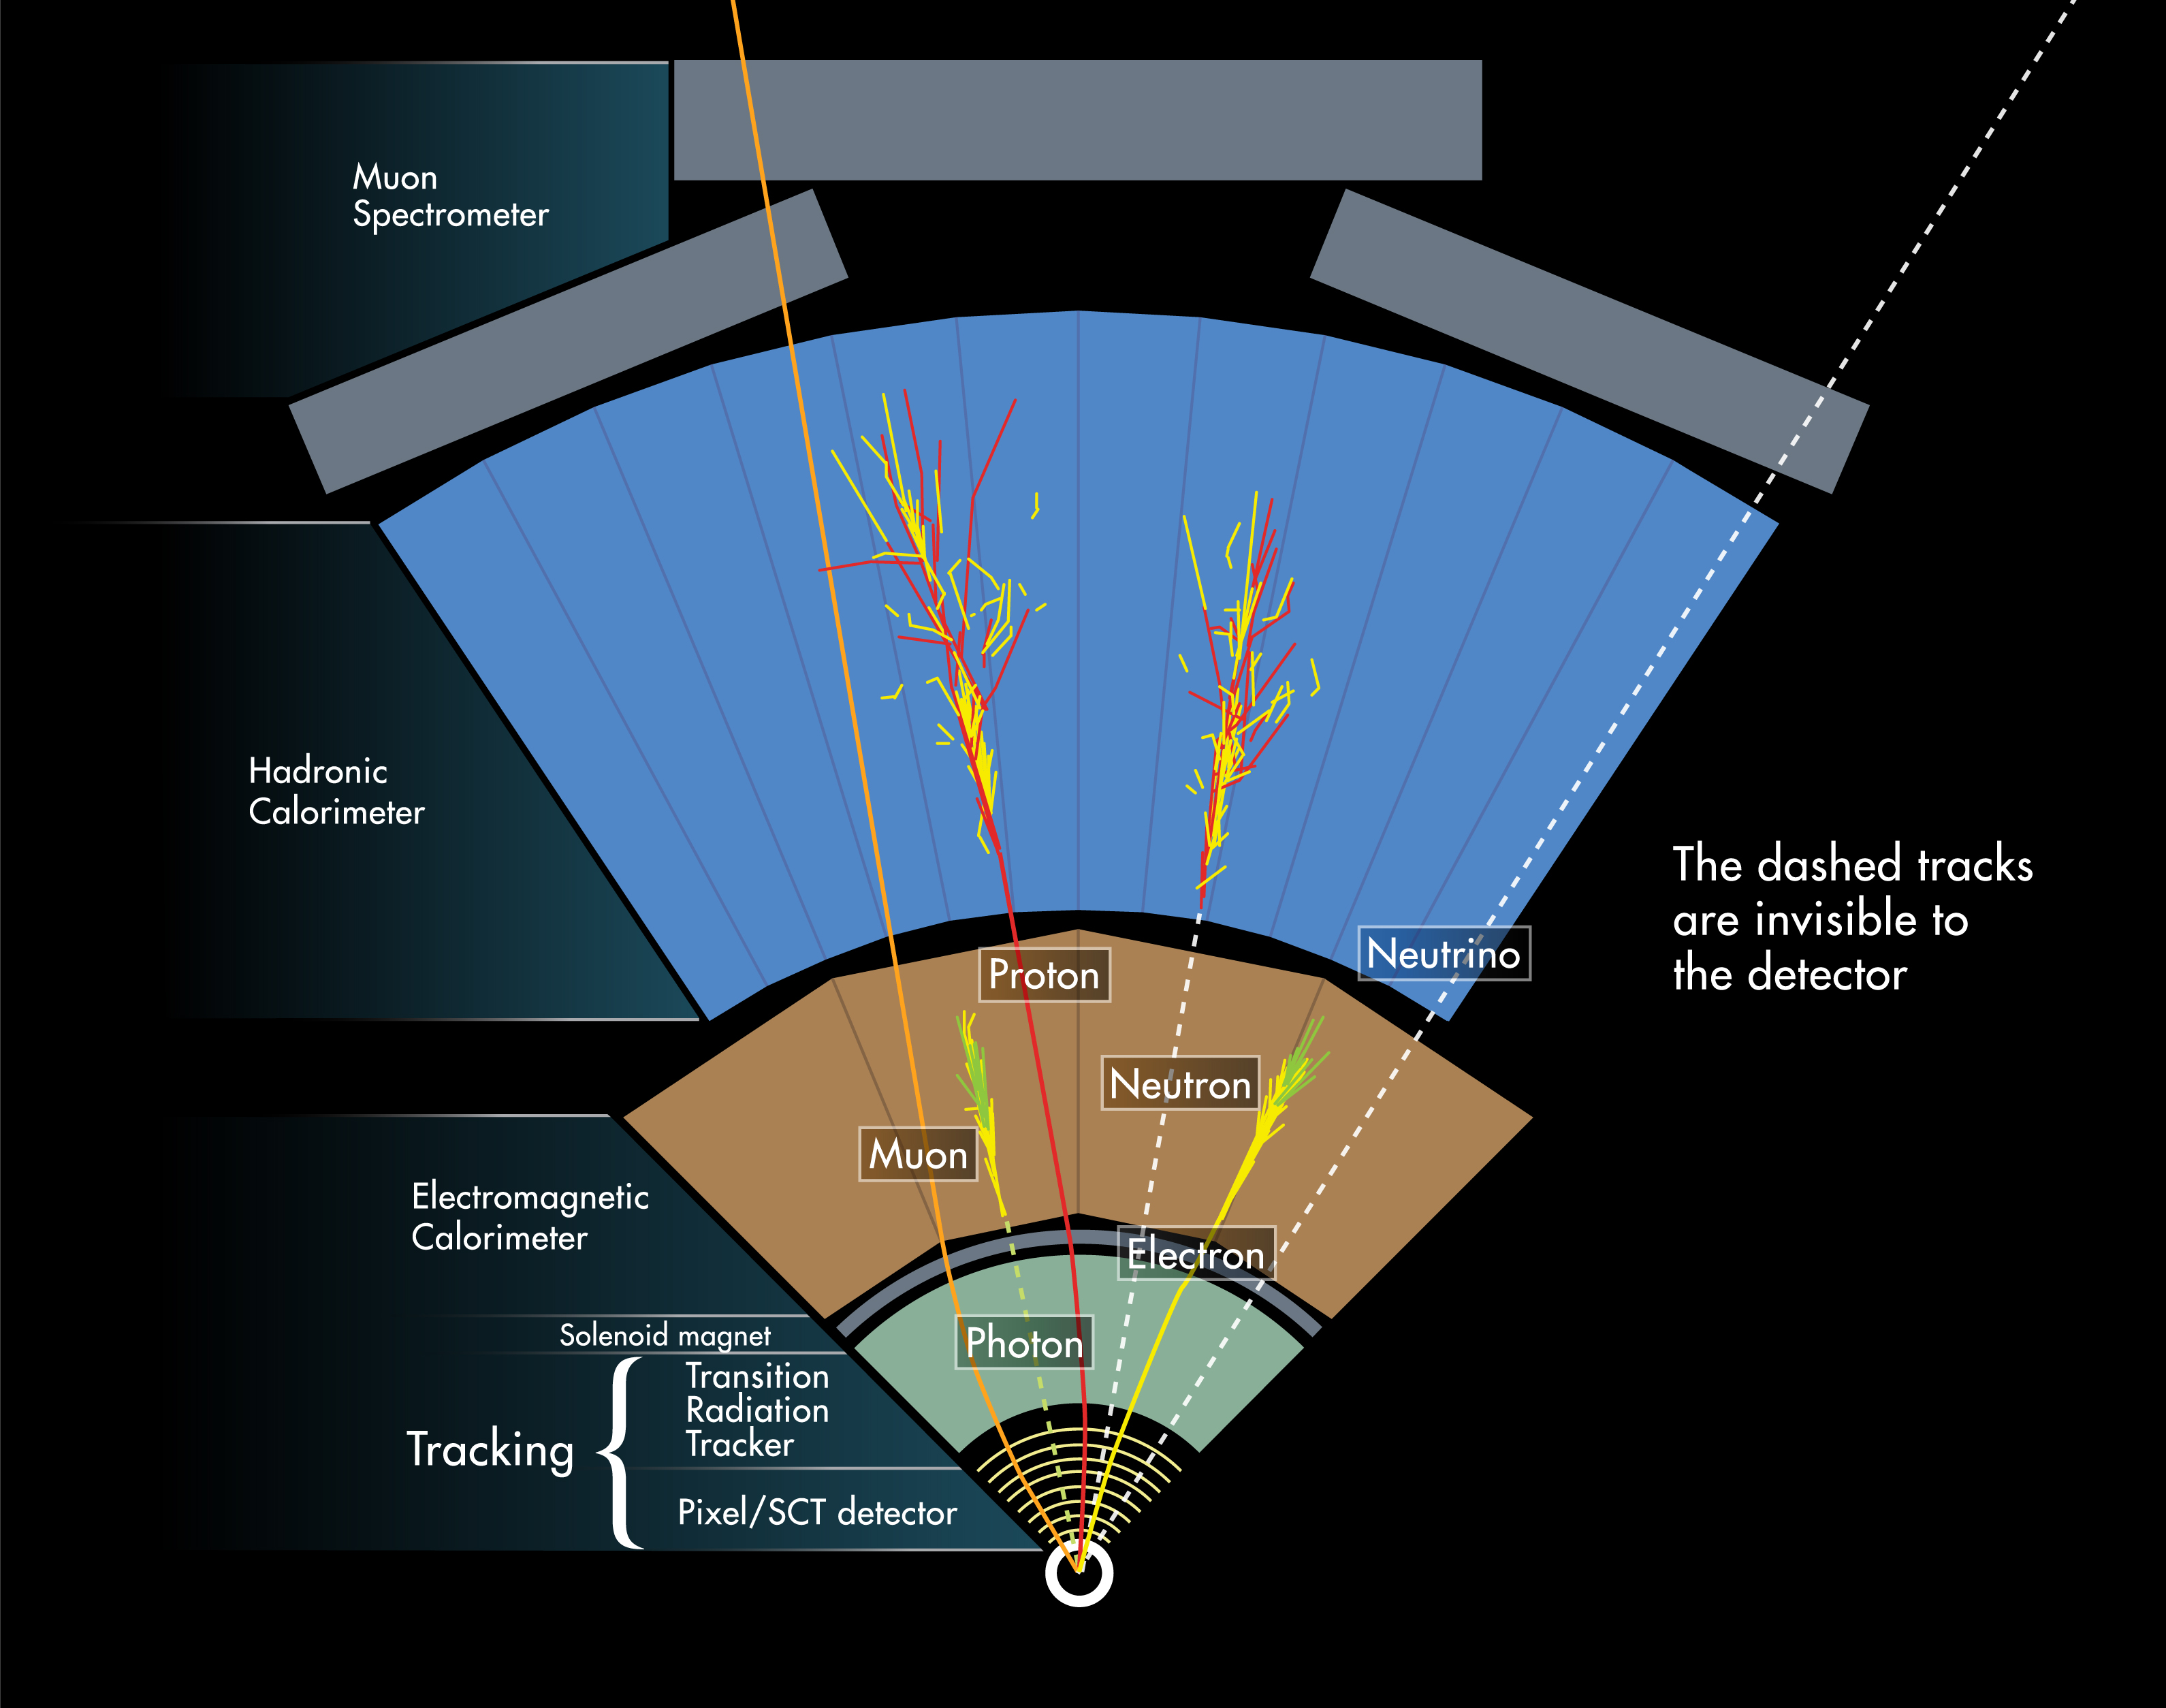
\includegraphics[width=\textwidth]{figs/lhc/particle_signatures.jpg}
  }
  \caption{
    Schematic view of the signatures left in the various sub-detectors of
    \atlas\ in response to the primary particles which pass through
    it~\cite{Pequenao:1505342}.
  }
  \label{fig:particle_signatures}
\end{figure}

%% - - - - - - - - - - - - - - - - - - - - - - - - - - - - - - - - - - - - - - -
\FloatBarrier
\subsection{Electrons} 
\label{sec:elctrons}

{\color{red} TODO Write about electrons}

%% - - - - - - - - - - - - - - - - - - - - - - - - - - - - - - - - - - - - - - -
\FloatBarrier
\subsection{Muons} 
\label{sec:muons}

{\color{red} TODO Write about electrons}

%% - - - - - - - - - - - - - - - - - - - - - - - - - - - - - - - - - - - - - - -
\FloatBarrier
\subsection{Jets} 
\label{sec:jets}

{\color{red} TODO this is the text from the CONF note. Update and expand...}

Jets are reconstructed using the anti-$k_{t}$
algorithm~\cite{Cacciari:2008gp, Cacciari:2005hq} with a radius
parameter $R = $ 0.4 from calibrated clusters of energy deposits in
the calorimeters. The differences in calorimeter response between
electrons, photons and hadrons are taken into account by classifying
each cluster, prior to the jet reconstruction, as coming from an
electromagnetic or hadronic shower on the basis of its shape
\cite{JES}.  The jet energy thus accounts for electromagnetic
and hadronic energy deposits at the cluster level with correction
factors derived from MC simulation.  A further correction,
used to calibrate the jet energy to the scale of its constituent
particles, (JES) \cite{JES,JES2}, is then applied.  The impact of
pileup is accounted for using
a technique, based on jet areas, that provides an event-by-event and
jet-by-jet correction \cite{Cacciari:2007fd}.  Jets are required
to have transverse momentum \pt\ $>$ 40~\GeV\ and $|\eta| < 4.9$.
In order to reduce contamination from jets produced by pileup,
the scalar sum of the \pt\ of the tracks matched to the jet and
originating from the primary vertex must be at least 50\% of the
scalar sum of the \pt\ of all tracks matched to the jet.  This
criterion is only applied to jets with $\pt < 50 \GeV$ and $|\eta| < 2.4$.

%% - - - - - - - - - - - - - - - - - - - - - - - - - - - - - - - - - - - - - - -
\FloatBarrier
\subsection{Flavor tagging} 
\label{sec:flavor_tagging}

{\color{red} TODO this is the text from the CONF note. Update and expand...}

The identification of $b$-jets uses the MV1 flavor tagging
algorithm~\cite{ATLAS-CONF-2014-004, ATLAS-CONF-2014-046}, which is
based on an artificial neural network
algorithm that exploits the impact parameters of charged particle
tracks, the parameters of reconstructed secondary vertices, and the
topology of $b$- and $c$-hadron decays inside a jet.  The operating
point corresponds to an overall 80\% $b$-tagging efficiency, as
measured in simulated \TTBAR\ events, a rejection factor of 25 for jets
originating from light quarks or gluons, and a rejection factor of
3 for jets originating from charm quarks.

%% - - - - - - - - - - - - - - - - - - - - - - - - - - - - - - - - - - - - - - -
\FloatBarrier
\subsection{Missing energy} 
\label{sec:met}

% {\color{red} missing momentum?}
{\color{red} TODO this is the text from the CONF note. Update and expand...}

The vector momentum imbalance in the transverse plane is obtained from
the negative vector sum of the reconstructed and calibrated physics
objects and the calorimeter energy clusters not associated with reconstructed
objects. This is denoted as missing transverse momentum, and the symbol
$\met$ is used for its magnitude.  The $\met$ calculation is described
elsewhere~\cite{ATLAS-CONF-2013-082}.
 
